\documentclass[notheorems,envcountsect,t,xcolor=table,aspectratio=169,draft,]{beamer}
\synctex=1
%draft
\includeonlyframes{bib,current}
%,notes=show
%,hyperref={bookmarks=true}
%trans
%beamer
%handout
%notes=hide/show/only

%\usepackage[usenames,dvipsnames]{xcolor}

%\newcommand{\nop}[1]{}
\newcommand{\nop}[1]{#1}
\usepackage{enumerate}

\usepackage[usestackEOL]{stackengine} % to use \Longstack
\usepackage{pifont}% http://ctan.org/pkg/pifont
\newcommand{\cmark}{\ding{51}}%
\newcommand{\xmark}{\ding{55}}%

\usepackage{array,etoolbox}
\preto\tabular{\setcounter{magicrownumbers}{-1}}
\newcounter{magicrownumbers}
\newcommand\rownumber{\stepcounter{magicrownumbers}\arabic{magicrownumbers}}

% TABLE EXTRAS
\usepackage{array}
\newcolumntype{H}{>{\setbox0=\hbox\bgroup}c<{\egroup}@{}}
\newcommand{\ts}[1]{\textit{#1}}
\newcommand{\tm}[1]{\textbf{#1}}


%fix to many includes
%"! No room for a new \dimen"
\usepackage{etex}


	\usepackage{listings}
	\usepackage{tikz}
	\usepackage{color}
	%\usepackage{soul}
	%\usepackage{adjustbox}
	\usepackage{colortbl}
	\usepackage{multicol}
	\usepackage{multirow}  % Allows table elements to span several rows.
	\usepackage{booktabs}  % Improves the typesettings of tables.

	%\usepackage{floatrow}
	% Table float box with bottom caption, box width adjusted to content
	%\newfloatcommand{capbtabbox}{table}[][\FBwidth]
	\newcommand{\blahtab}[1]{{\tiny{#1}}}%
	%\usepackage{blindtext}
	\newcommand{\parhead}[1]{\smallskip\noindent\textbf{#1}\ }				

	%\usepackage{memoir}
	%\usepackage{appendixnumberbeamer}
	%>>>
	%<<< Set up listings

	\newcommand{\inputPredColor}{purple!70!black}
	\newcommand{\outputPredColor}{orange!70!black}
	\newcommand{\specialTermColor}{blue!70!black}
	\definecolor{dkgreen}{rgb}{0,0.5,0}
	%\setstcolor{\specialTermColor}
	%\setstcolor{\specialTermColor}
	%\sethlcolor{\specialTermColor}
	\definecolor{gyellow}{rgb}{1.0, 0.97, 0.33}
	\definecolor{mygreen}{RGB}{0,192,0}
	\definecolor{myblue}{RGB}{40,40,255}
	\definecolor{myorange}{RGB}{253,126,0}

	\definecolor{HighlightColor}{rgb}{1.0, 0.97, 0.33}
	%\definecolor{HighlightColor}{rgb}{1.0, 0.5, 0}
	%\definecolor{HighlightColor}{rgb}{0.13,0.67,0.8}
	\makeatletter
	\def\rowcolor{\noalign{\ifnum0=`}\fi\bmr@rowcolor}
	\newcommand<>{\bmr@rowcolor}{%
	    \alt#1%
		{\global\let\CT@do@color\CT@@do@color\@ifnextchar[\CT@rowa\CT@rowb}% 
		{\ifnum0=`{\fi}\@gooble@rowcolor}% 
	}

	\newcommand{\@gooble@rowcolor}[2][]{\@gooble@rowcolor@}
	\newcommand{\@gooble@rowcolor@}[1][]{\@gooble@rowcolor@@}
	\newcommand{\@gooble@rowcolor@@}[1][]{\ignorespaces}
	\makeatother

	\newcommand{\predicate}[1]{\texttt{\small #1}}

	\lstdefinelanguage{dflat}{
	    firstnumber=1, % XXX Workaround because otherwise warnings occur with hyperref
	    otherkeywords={:-},
	    morekeywords={not},
	    keywordstyle=\sffamily\bfseries,
	%    emph={root,childNode,current,introduced,removed,childRow,sub,childItem,childCount,childCost,item,extend,count,cost,currentCost,levels,optItem},
	    emph={final,childNode,current,introduced,removed,childRow,sub,childItem,childCount,childCost,childAuxItem,bag, atNode, rootOf, root},
	    moreemph=[2]{item,extend,count,cost,currentCost,levels,optItem,auxItem , reject, accept, or, and, length},
	    moreemph=[3]{pos, neg, att, head, p, clause, atom, z, sim, cor,minimize, fix},
	    moreemph=[4]{},%out, in, outc, def, defc},
	    alsoletter={\#}, % This is required to avoid coloring, e.g., the #count aggregate because it is mistakenly interpreted as the count/1 predicate
	%    emphstyle=\rmfamily,
	%    emphstyle=[2]\slshape,
	    emphstyle=\color{\inputPredColor},
	    emphstyle=[2]\color{\outputPredColor},
	    emphstyle=[3]\color{\specialTermColor},
	    emphstyle=[4]\color{\decompositionColor},
	    morecomment=[l]{\%},
	    commentstyle=\rmfamily\small\itshape\color{dkgreen},
	    %numbers=left,
	    numbersep=1pt,                  % how far the line-numbers are from the code
	    numberstyle=\tiny\color{gray},
	    numberblanklines=false,
	   % flexiblecolumns=true,
	    %columns=fullflexible,
	%    lineskip=1mm,
	    literate={:-}{{$\la$}}2 {!=}{{$\neq$}}1,
	    breakindent=20pt,
	    escapechar=@, % Useful, e.g., for manually breaking lines via @\\@
	}
	\lstset{%
		aboveskip=0mm,
		belowskip=0mm,
		basicstyle=\footnotesize\ttfamily,
		tabsize=4,
		breaklines=true,
		breakatwhitespace=true,
		fontadjust,
		language=dflat,
	    %firstnumber=1,%
	}
	%>>>
	%<<< Set up TikZ


\lstdefinelanguage{dflat}{
    firstnumber=1, % XXX Workaround because otherwise warnings occur with hyperref
    otherkeywords={:-},
    morekeywords={not},
    keywordstyle=\sffamily\bfseries,
%    emph={root,childNode,current,introduced,removed,childRow,sub,childItem,childCount,childCost,item,extend,count,cost,currentCost,levels,optItem},
    emph={final,childNode,current,introduced,removed,childRow,sub,childItem,childCount,childCost,childAuxItem,bag, atNode, rootOf, root},
    moreemph=[2]{item,extend,count,cost,currentCost,levels,optItem,auxItem , reject, accept, or, and, length},
    moreemph=[3]{pos, neg, att, head, p, clause, atom, z, sim, cor,minimize, fix},
    moreemph=[4]{},%out, in, outc, def, defc},
    alsoletter={\#}, % This is required to avoid coloring, e.g., the #count aggregate because it is mistakenly interpreted as the count/1 predicate
%    emphstyle=\rmfamily,
%    emphstyle=[2]\slshape,
    emphstyle=\color{\inputPredColor},
    emphstyle=[2]\color{\outputPredColor},
    emphstyle=[3]\color{\specialTermColor},
    emphstyle=[4]\color{\decompositionColor},
    morecomment=[l]{\%},
    commentstyle=\rmfamily\small\itshape\color{dkgreen},
    %numbers=left,
    numbersep=1pt,                  % how far the line-numbers are from the code
    numberstyle=\tiny\color{gray},
    numberblanklines=false,
   % flexiblecolumns=true,
    %columns=fullflexible,
%    lineskip=1mm,
    literate={:-}{{$\la$}}2 {!=}{{$\neq$}}1,
    breakindent=20pt,
    escapechar=@, % Useful, e.g., for manually breaking lines via @\\@
}
\lstset{%
	aboveskip=0mm,
	belowskip=0mm,
	basicstyle=\footnotesize\ttfamily,
	tabsize=4,
	breaklines=true,
	breakatwhitespace=true,
	fontadjust,
	language=dflat,
    %firstnumber=1,%
}
%>>>
%<<< Set up TikZ
\usetikzlibrary{arrows,automata,shapes,calc,shadows,positioning,fit,decorations.pathreplacing}
%\usetikzlibrary{external}
%\tikzexternalize[prefix=external-figures/]

%http://tex.stackexchange.com/questions/117873/add-a-curved-arrow-and-a-bracket-to-a-table
\newcommand{\tikzmark}[2][-3pt]{\tikz[remember picture, overlay, baseline=-0.5ex]\node[#1](#2){};}
\newcounter{arrow}
\setcounter{arrow}{0}
\newcommand{\drawcurvedarrow}[3][]{%
 \refstepcounter{arrow}
 \tikz[remember picture, overlay]\draw (#2.center)edge[#1]node[coordinate,pos=0.5, name=arrow-\thearrow]{}(#3.center);
}

\tikzstyle{cc}=[color=red,thin,->,>=to]
\tikzstyle{tdnode} = [draw,rounded corners,minimum size=1.1em, font=\small, prefix after command={\pgfextra{\tikzset{every label/.style={font=\small, label distance=-0.1cm}}}},
left color=blue!10!gray!10, right color=blue!30!gray!10, middle color=white]
\tikzstyle{tdedge} = [-,thick]
\tikzstyle{itemtreed1} = [level 1/.style={sibling distance = 3.7em}, level distance = 2.0em]
\tikzstyle{itemtreed1small} = [level 1/.style={sibling distance = 2.7em}, level distance = 2.9em]
\tikzstyle{itemtree} = [level 1/.style={sibling distance = 5.1em}, level 2/.style={sibling distance = 3.3em}, level distance = 2em]
\tikzstyle{itrootnode} = [draw,circle, minimum size=0.4em, left color=white, right color=white, middle color=white]
\tikzstyle{itnode} = [draw,rounded corners,minimum size=1.5em, node distance=0.7em, left color=red!10, right color=red!25, middle color=white]
\tikzstyle{extensionpointer} = [->, densely dashed, scale=0.7]
\tikzstyle{extensionpointerback} = [extensionpointer, <->]
\tikzstyle{counterpointer} = [->, solid, scale=0.7]
\tikzstyle{highlight} = [red,thick]
\tikzstyle{arrowstyle}=[arrowfill, single arrow, inner sep=0.3em, yscale=0.5, single arrow, single arrow head extend=.25em]
\tikzstyle{arrowfill}=[top color=red!50, bottom color=red!80]%, general shadow={fill=black, shadow yshift=-0.8ex, path fading=arrowfading}]
\tikzstyle{coderef}=[fill=white,shape=circle, inner sep=0, outer sep=0, font=\small]%, text=black]
\tikzstyle{argument}=[circle,fill=white,draw=black,thin,minimum size=9mm]
\tikzstyle{ptr}=[draw,rectangle,minimum height=0.25cm,minimum width=0.25cm]
\tikzstyle{extpointer}=[->,dashed,>=latex]

\tikzstyle{gnode} = [draw, circle, node distance=0.2em, inner sep=1.5pt, outer sep=0pt, minimum size=0.8em]%, font=\scriptsize]

\tikzstyle{bddnode} = [draw, rectangle, rounded corners=0.1em, minimum size=1.15em, inner sep=0, font=\scriptsize, left color=yellow!10, right color=yellow!10, middle color=yellow!10]
\tikzstyle{bddepos} = [->,solid]
\tikzstyle{bddeneg} = [->,densely dashed]
\tikzstyle{tdnodetab} = [tdnode,
left color=green!30!gray!10, right color=green!30!gray!10, middle color=green!30!gray!10]

\tikzstyle{rect1} = [fill=blue!30,rounded corners=2pt]
\tikzstyle{rect2} = [fill=blue!10,rounded corners=2pt]
\tikzstyle{rect3} = [gray!60, fill=gray!10, rounded corners=2pt]




%\tikzfading[name=fade south, top color=transparent!0, bottom color=transparent!100]

\tikzset{
	%auto,
	%font=\scriptsize,
	% Cf. http://tex.stackexchange.com/questions/6135/how-to-make-beamer-overlays-with-tikz-node
	onslide/.code args={<#1>#2}{%
		\only<#1>{\pgfkeysalso{#2}}
	}
}

\tikzstyle{subway}=[
	font=\tiny,
	rounded corners=2pt,
	subwayedge/.style={line width=1.4mm},
	u1/.style={subwayedge,draw=red},
	u2/.style={subwayedge,draw=violet},
	u3/.style={subwayedge,draw=orange},
	u4/.style={subwayedge,draw=green!70!black},
	u6/.style={subwayedge,draw=brown},
	station/.style={circle,draw,line width=0.8pt,fill=white, outer sep=0pt, inner sep=3pt},
	smallstation/.style={rectangle, inner sep=0, outer sep=0pt, minimum height=3mm, minimum width=1.5mm, sharp corners},
	u1station/.style={smallstation,fill=red},
	u2station/.style={smallstation,fill=violet},
	u3station/.style={smallstation,fill=orange},
	u4station/.style={smallstation,fill=green!70!black},
	u6station/.style={smallstation,fill=brown},
	sname/.style={inner sep=0pt, outer sep=0pt},
	sname spaced/.style={},
%	solution/.style={draw=black,top color=black,bottom color=black!50,line width=0.8pt,double},
]

\tikzstyle{subwayscaled}=[
	subway,
	scale=0.5,
	every node/.style={transform shape},
	subwayedge/.style={line width=0.7mm},
	station/.style={circle,draw,line width=0.6pt,fill=white, outer sep=0pt, inner sep=3pt},
%	solution/.style={draw=black,top color=black,bottom color=black!50,line width=0.4pt,double},
	solution/.style={},
]

\tikzstyle{subwaytiny}=[
	subway,
	scale=0.4,
	every node/.style={transform shape},
	subwayedge/.style={line width=0.56mm},
	station/.style={circle,draw=black,line width=0.48pt,fill=white, outer sep=0pt, inner sep=3pt},
	solution/.style={},
]

\newcommand{\vertexTopColor}{white}
\newcommand{\vertexBottomColor}{blue!20!black!15}
\tikzstyle{vertex}=[%
	draw,
	circle,
	minimum size=6mm,
	top color=\vertexTopColor,
	bottom color=\vertexBottomColor,
	]
\tikzstyle{tdnode}=[%
	draw,
	rounded corners,
	top color=\vertexTopColor,
	bottom color=\vertexBottomColor,
	]
%>>>
%<<< Macros to use as shortcuts


	\newcommand{\attacks}{\rightarrowtail}
	\renewcommand{\O}{\ensuremath{\mathcal{O}}}
	\renewcommand{\implies}{\ensuremath{\supset}}
	\newcommand{\pred}[1]{\texttt{#1}}
	\newcommand{\problemname}[1]{\textsc{#1}}
	\newcommand{\threeCol}{\problemname{$3$-Col}} % The figure 3 is set in math mode because loading, e.g., mathpazo with the osf option would set the 3 as a text figure (cf. wikipedia) which looks odd in small caps.
	\newcommand{\minCol}{\problemname{Minimal $3$-Coloring}}
	\newcommand{\sat}{\problemname{Sat}}
	\newcommand{\qsat}{\problemname{Qsat}}
	\newcommand{\threeSat}{\problemname{$3$-Sat}}
	\newcommand{\twoSat}{\problemname{$2$-Sat}}
	\newcommand{\hamCycle}{\problemname{Hamiltonian Cycle}}
	\newcommand{\vertexCover}{\problemname{Vertex Cover}}
	\newcommand{\mvc}{\problemname{Minimum Vertex Cover}}
	\newcommand{\cyclicOrdering}{\problemname{Cyclic Ordering}}
	\newcommand{\msoFormulaEvaluation}{\problemname{Mso Formula Evaluation}}
	\newcommand{\mids}{\problemname{Minimum Independent Dominating Set}}
	\newcommand{\complexityclass}[1]{\ensuremath{\mathsf{#1}}}
	\let\defaultP\P
	\renewcommand{\P}{\complexityclass{P}}
	\newcommand{\NP}{\complexityclass{NP}}
	\newcommand{\PH}{\complexityclass{PH}}
	\newcommand{\Pspace}{\complexityclass{PSPACE}}
	\newcommand{\Sp}[1]{\ensuremath{\Sigma^p_{#1}}}
	\newcommand{\Pp}[1]{\complexityclass{\Pi^p_{#1}}}
	\newcommand{\Dp}[1]{\complexityclass{\Delta^p_{#1}}}
	%\newcommand{\co}{\complexityclass{co-}}
	\mathchardef\mhyphen="2D
	\newcommand{\co}{\complexityclass{co\mhyphen}}
	\newcommand{\sizeof}[1]{\ensuremath{\lvert #1 \rvert}}
	\newcommand{\dneg}{\ensuremath{\operatorname{not}\,}}
	\newcommand{\dflat}{\mbox{D-FLAT}}
	\newcommand{\A}{\ensuremath{\mathcal{A}}}
	%\renewcommand{\phi}{\varphi}
	%\newcommand{\undef}{\ensuremath{\textrm{undef}}}


	%\newcommand{\pname}[1]{\mathrm{\rmfamily\scshape #1}} % \textsc{#1}\xspace}
	\newcommand{\pname}[1]{{#1}} % \textsc{#1}\xspace}
	%\newcommand{\problem}[1]{\textsc{#1}}
	\newcommand{\Sat}{\problemname{Sat}}
	\newcommand{\MinSat}{\problemname{$k,\subseteq$-Minimal Sat}}
	\newcommand{\MaxSat}{\problemname{MaxSat}}
	\newcommand{\Circ}{\problemname{Circ}}


\newcommand{\BigO}[1]{\ensuremath{\mathcal{O}(#1)}}
\newcommand{\Card}[1]{|#1|}

\mode<presentation>
{
  % \usetheme{default}
  \usetheme{DRM}
  % \useoutertheme{infolines}
  \usecolortheme{rose}
  \setbeamercolor{block title}{fg=DRMBlue,bg=}

  % \setbeamertemplate{navigation symbols}{}
  \setbeamertemplate{blocks}[rounded]
  %\addtobeamertemplate{block begin}{\pgfsetfillopacity{0.5}}{\pgfsetfillopacity{1}}
  \setbeamertemplate{footline}[frame number]{}
  \setbeamercolor{structure}{fg=blue!40!gray!50!black}
  \setbeamercolor{example text}{fg=green!50!gray!60!black}
  %	\setbeamercolor{block title}{bg=blue!20!gray!25}
  %	\setbeamercolor{block title example}{bg=green!25!gray!40}
}

%\newcommand{\tikzmark}[1]{\tikz[overlay,remember picture] \node (#1) {};}


%===================================================================
%		Basic Stuff
%===================================================================
\usepackage{xspace}
\usepackage{amssymb}% http://ctan.org/pkg/amssymb
\usepackage{amsmath}
\usepackage{mathtools}
\usepackage{url}
\usepackage{xspace}
\usepackage{setspace} 
\usepackage{mathtools}

\newcommand{\F}[1]{F^{\mathit{#1}}}
\DeclareMathAlphabet{\mathpzc}{OT1}{pzc}{m}{it}
\DeclareMathOperator{\width}{width}


\usepackage{bbding}
\usepackage{listings}
\lstset{basicstyle=\ttfamily, escapechar=\%}
%\usepackage{enumitem}

\newcommand{\pvar}[1]{\ensuremath{{\text{#1}}}}
\newcommand{\FSkept}{F_{\text{Caut}}}
\newcommand{\FBrave}{F_{\text{Brave}}}

\newcommand{\eqdef}{\ensuremath{\,\mathrel{\mathop:}=}}
\newcommand{\cid}[1]{\ensuremath{[\![#1]\!]}}
\DeclareMathOperator{\attr}{att}


%===================================================================
%		Algorithms
%===================================================================
%\usepackage[ruled,linesnumbered,noend,noline]{algorithm2e}

\usepackage{cancel}

\usepackage{docmute}
\makeatletter
\newcommand*{\loadpresentation}[1]{{\beamer@inlecturefalse\input{#1}}}
\makeatother


\usepackage{tabularx}

%===================================================================
%		Math Symbols
%===================================================================
\usepackage{amsmath,amssymb,amsthm}
\newtheorem{LEM}{Lemma} 
\newtheorem{THE}{Theorem} 
\newtheorem{OBS}{Observation} 
\newtheorem{corollary}{Corollary} 
\newtheorem{CLM}{Claim} 
\newtheorem{proposition}{Proposition} 
\newtheorem{definition}{Definition} 
\newtheorem{REM}{Remark} 

\newtheorem{EXAMPLE}{Example} 
 
\def\hy{\hbox{-}\nobreak\hskip0pt} 
\newcommand{\ellipsis}{$\dots$}
\newcommand{\SB}{\{\,}%
\newcommand{\SM}{\;{:}\;}%
\newcommand{\SE}{\,\}}%
\newcommand{\SBb}{\big\{\,}%
\newcommand{\SEb}{\,\big\}}%
 
\newcommand{\seq}[1]{\langle #1 \rangle}
\newcommand{\QB}{\langle\,}%
\newcommand{\QM}{\;{:}\;}%
\newcommand{\QE}{\,\rangle}%

\newcommand{\ra}{\ensuremath{\rightarrow}}
\newcommand{\Ra}{\ensuremath{\Rightarrow}\xspace}
\newcommand{\la}{\leftarrow}


%\newcommand{\Card}[1]{|#1|}
\newcommand{\CCard}[1]{\|#1\|}
\newcommand{\size}[1]{\|#1\|}

%\let\phi=\varphi
\let\epsilon=\varepsilon

\newcommand{\UP}{\text{\normalfont{UP}}}
\newcommand{\Nat}{\mathbb{N}}
 
\newcommand{\AAA}{\mathsf{A}} 
\newcommand{\HHH}{\mathsf{H}}
%\newcommand{\SSS}{\mathsf{S}}
\newcommand{\SSS}{\mathcal{S}}
\newcommand{\BBB}{\mathcal{B}}
\newcommand{\CCC}{\ensuremath{\mathcal{C}}}
\newcommand{\LLL}{\mathcal{L}} \newcommand{\FFF}{\mathcal{F}}
\newcommand{\GGG}{\mathcal{G}} 
\newcommand{\MMM}{\mathcal{M}} \newcommand{\PPP}{\mathcal{P}}
\newcommand{\QQQ}{\mathcal{Q}} \newcommand{\RRR}{\mathcal{R}}
 \newcommand{\TTT}{\mathcal{T}}
\newcommand{\VVV}{\mathcal{V}}
\newcommand{\bigoh}{\mathcal{O}}

\newcommand{\mtext}[1]{\text{\normalfont #1}}
\newcommand{\btext}[1]{\text{\normalfont\bfseries #1}}

\newcommand{\rel}{\mathit{rel}}
\newcommand{\var}{\mathit{var}}
\newcommand{\eovl}{\mathit{ovl}^*}
\newcommand{\cmp}{\mathit{cmp}}
\newcommand{\nil}{\mathnormal{\square}}

\newcommand{\ol}[1]{\overline{#1}}
\newcommand{\pair}[1]{\langle #1 \rangle}

\newcommand{\ComplClass}[1]{\text{\normalfont #1}\xspace}
\renewcommand{\L}{\text{\normalfont L}}
\newcommand{\SharpP}{\#P}
\newcommand{\LOGSPACE}{\text{\normalfont logspace}}
\renewcommand{\P}{\text{\normalfont P}\xspace}
\newcommand{\coNP}{\text{\normalfont co-NP}\xspace}
\newcommand{\coNPp}{\text{\normalfont co-NP/poly}\xspace}
\newcommand{\NPp}{\text{\normalfont NP/poly}\xspace}
\newcommand{\NCp}[1][xxxx]{\ensuremath{\text{\normalfont NC}^{#1}}{\text{/\normalfont{poly}}}\xspace}
\newcommand{\PSPACE}{\text{\normalfont PSPACE}\xspace}
\newcommand{\FPT}{\text{\normalfont FPT}\xspace}
\newcommand{\XP}{\text{\normalfont XP}\xspace}
\newcommand{\W}[1][xxxx]{\text{\normalfont W[#1]}\xspace}
\newcommand{\para}[1]{\ensuremath{\mtext{para\hy #1}}}
\newcommand{\paraNP}{\text{\normalfont para\hy NP}\xspace}
\newcommand{\coparaNP}{\text{\normalfont co-para\hy NP}\xspace}
\newcommand{\paracoNP}{\text{\normalfont para\hy co\hy NP}\xspace}
\newcommand{\paraSigmaP}{\para{\ensuremath{\Sigma^P_2}}}

%\newcommand{\BigO}[1]{\ensuremath{\mathcal{O}(#1)}}
%\newcommand{\PR}[2]{\text{\normalfont\textsc{\bfseries #1}(#2)}}

\newcommand{\stableset}{\text{\normalfont AS}}
\newcommand{\at}{\text{\normalfont at}}

\newcommand{\ta}[1]{\text{\normalfont ta($#1$)}}
\newcommand{\rsep}{;\;}


\newcommand{\class}[1]{{\bf #1\normalfont}}
\newcommand{\parm}[1]{\textnormal{#1}}

\newcommand{\NSTR}{\class{Strat}}
\newcommand{\lc}{\text{lc}}
\newcommand{\cwd}{\text{cwd}}

\newcommand{\pmm}[3]{\ensuremath{{#1}|^{#2}_{#3}}}
\newcommand{\pmmt}[3]{\ensuremath{{#1}{\downarrow^{#2}_{#3}}}}


\newcommand{\AspBrave}{\pname{Brave Reasoning}}
\newcommand{\kAspBrave}{$k$\hy \pname{Brave Reasoning}}
\newcommand{\kAspCaut}{$k$\hy \pname{Skeptical Reasoning}}
\newcommand{\kAspReason}{\ensuremath{k\hy\mathpzc{AspReason}}\xspace}

\newcommand{\AspCheck}{\pname{Checking}}
\newcommand{\AspCons}{\pname{Consistency}}
\newcommand{\AspCaut}{\pname{Skeptical Reasoning}}
\newcommand{\AspCount}{\pname{Counting}}
\newcommand{\AspEnum}{\pname{Enum}}
\newcommand{\AspReason}{\ensuremath{\mathpzc{AspReason}}\xspace}
\newcommand{\AspFull}{\ensuremath{\mathpzc{AspFull}}\xspace}
\newcommand{\Bound}{\pname{Bound}}

\newcommand{\kAspCheck}{$k$\hy \pname{Checking}}
\newcommand{\kAspCons}{$k$\hy \pname{Consistency}}
\newcommand{\kAspEnum}{$k$\hy \pname{Enum}}


\newcommand{\Acyc}{\class{Acyc}}
\newcommand{\DAcyc}{\class{D-Acyc}}
\newcommand{\BAcyc}{\class{Bad-Acyc}}



\newcommand{\reduct}[2]{\ensuremath{#1_{#2}}}
\newcommand{\fvs}[0]{\text{\bfseries fvs}}
\newcommand{\tw}{\text{\normalfont tw}}

\newcommand{\pnot}{\neg}
\newcommand{\por}{\vee}

\newcommand{\NAT}{\mathbb{N}}



\newcommand{\pproblem}[4]{
\begin{quote}
\begin{samepage}
{\scshape {#1}\nopagebreak[4]} \normalfont \vspace{0.4em}\nopagebreak[4]\\
\begin{tabular}{lp{0.75\textwidth}}
  \emph{Given:} & #2 \tabularnewline[1pt]
 \emph{Parameter:} & #3 \tabularnewline[1pt]
  \emph{Task:} & #4 \tabularnewline[1pt]
\end{tabular}
\end{samepage}
\end{quote}
}


\usepackage{graphicx}


%\usepackage[ruled,vlined]{algorithm2e}
\usepackage[ruled,vlined,linesnumbered]{algorithm2e}
\newcommand*{\algorithmcfnameold}{Algorithm}
\newcommand*{\algorithmcfnamenew}{Listing}
\renewcommand*{\algorithmcfname}{\algorithmcfnameold}
\SetKwInput{KwData}{In}
\SetKwInput{KwResult}{Out}
\setlength{\textfloatsep}{1em}
\SetAlFnt{\small}
\SetAlCapFnt{\small}
\SetAlCapNameFnt{\small}
\SetAlCapHSkip{0pt}
\SetEndCharOfAlgoLine{}
\IncMargin{-0.4em}
\makeatletter
\newcommand{\algorithmfootnote}[2][\footnotesize]{
  \let\old@algocf@finish\@algocf@finish
  \def\@algocf@finish{\old@algocf@finish
    \leavevmode\rlap{\begin{minipage}{\linewidth}
    #1#2
    \end{minipage}}
  }
}
\makeatother
%
\newcommand{\tuplecolor}[1]{\textcolor{#1}}
\newcommand{\statePredColor}{green!62!black}
\newcommand{\specialPredColor}{red!62!black}
\newcommand{\tab}[1]{\ensuremath{\tau_{#1}}}

\DeclareMathOperator{\type}{type}
\newcommand{\intr}{\textit{intr}}
\newcommand{\leaf}{\textit{leaf}}
\newcommand{\rem}{\textit{rem}}
\newcommand{\join}{\textit{join}}


\usepackage{caption}

\usepackage{booktabs}
%===================================================================
%		Text Symbols
%===================================================================
\newcommand{\SAT}{\text{SAT}\xspace}
\newcommand{\UNSAT}{\text{UNSAT}\xspace}
\newcommand{\ASP}{\text{ASP}\xspace}
\newcommand{\QBFSAT}{\text{QBFSAT}\xspace}


\newcommand{\problem}[1]{\itshape #1}

\newcommand{\delBds}[1]{deletion {\ensuremath{#1}}\hy backdoor}
\newcommand{\strongBds}[1]{{strong \ensuremath{#1}}-backdoor}
\renewcommand{\problem}[1]{#1}

\newcommand{\MinCheck}{\textit{MinCheck}\xspace}
\newcommand{\AlgTrue}{\textit{True}\xspace}
\newcommand{\AlgFalse}{\textit{False}\xspace}
\newcommand{\BdBrave}[1]{\problem{\ensuremath{#1}-Back\-door\hy Brave\hy Rea\-son\-ing}}
\newcommand{\BdSkept}[1]{\problem{\ensuremath{#1}-Back\-door\hy Skeptical\hy Rea\-son\-ing}} 
\newcommand{\BdCheck}[1]{\problem{\ensuremath{#1}-Back\-door\hy Asp\hy Check}}
\newcommand{\BdDetect}[2]{\problem{#1 \ensuremath{#2}-Back\-door-De\-tec\-tion}}
\newcommand{\Normal}{\textbf{Normal}\xspace}
\newcommand{\DNormal}{\textbf{Dual-Normal}\xspace}
\newcommand{\Horn}{{\textbf{Horn}\xspace}}
\newcommand{\Strat}{{\textbf{Strat}\xspace}}
\newcommand{\Tight}{{\textbf{Tight}\xspace}}
\newcommand{\DHorn}{{\textbf{dual Horn}}\xspace}
\newcommand{\HCF}{{\textbf{HCF}}\xspace}

\newcommand{\gs}{\parm{gs}}
\newcommand{\psize}{\parm{size}}
\newcommand{\numleaves}{\parm{\#leaves}}
\newcommand{\bdTree}[1]{{\ensuremath{#1}}\hy back\-door tree}
\newcommand{\BdTreeComp}[1]{#1\hy\textsc{BdTreeComp}}
\newcommand{\BdTreeCheck}[1]{\pname{\ensuremath{#1}-Back\-door Tree Asp Check}}
\newcommand{\GalloScutella}{Gallo-Scutell\`a\xspace}

\newcommand{\lrsep}{}
\newcommand{\tight}{\text{\bfseries Tight}\xspace}



%===================================================================
%		Slides
%===================================================================
\mode<presentation>{\usetheme{DRM}}
 

\usepackage{subfig}
%\usepackage{multicol}
%Hyphenation in Beamer Slides
%\usepackage{ragged2e}
%\let\raggedright=\RaggedRight

\setbeamercovered{transparent}


\usepackage[absolute,overlay]{textpos}
\usepackage{graphicx}

%===================================================================
%		Fonts
%===================================================================	
\usepackage{xltxtra}
% %\usepackage{fontspec}
% % \setmainfont{OpenSans-Light}
% %\setmainfont{TU Text Light}
% % \setmainfont[
% %    ItalicFont     = TU Text LightItalic,
% %    BoldFont       = TU Text Regular,
% %    BoldItalicFont = TU Text RegularItalic]{TuText}
% % \newfontfamily\NHLight[
% %    ItalicFont     = TU Text LightItalic,
% %    BoldFont       = TU Text Medium,
% %    BoldItalicFont = TU Text MediumItalic]{TuText-Light}

% \usepackage{xltxtra,fontspec,xunicode}
% \defaultfontfeatures{Scale=MatchLowercase}
% %%\setromanfont[Numbers=Uppercase]{TU Text Regular}
% \setromanfont[Numbers=Uppercase]{TU Headline Regular}
% \setsansfont[Numbers=Uppercase]{TU Text Light}
% %%\setmonofont[Scale=0.90,Ligatures=NoCommon]{Courier}


% %\setromanfont[Numbers=Uppercase]{OpenSans-SemiBold}
% %\setsansfont[Numbers=Uppercase]{OpenSans-Light}


%\usepackage{bold-extra}
%\renewcommand*{\rmdefault}{pfr}
%\renewcommand{\sfdefault}{pfr}
\renewcommand{\seriesdefault}{l}
% \renewcommand*{\rmdefault}{cmr}
% \renewcommand{\sfdefault}{cmr}
%\usepackage{frutiger}          
%\renewcommand<>{\emph}[1]{{\only#2{\itshape}#1}}

%{\sffamily}
%\DeclareFontShape{OT1}{pfr}{l}{sc} { <-> sub * OMS/phy/n/sc }{}
%\DeclareFontShape{OT1}{pfr}{l}{sc} { <-> sub * cmsy/m/n }{}


%===================================================================
%		PDF Hyperlinks
%===================================================================
\definecolor{links}{HTML}{2A1B81}
%\hypersetup{colorlinks,linkcolor=,urlcolor=links}

%===================================================================
%		Bibliography
%===================================================================
\usepackage{url}\urlstyle{rm}
\bibliographystyle{alpha}
%\newcommand{\bcite}[1]{\textcolor{blue}{[#1]}}
\newcommand{\bcite}[1]{\alert{[#1]}}

%\newcommand{\citeauthoryear}[2]{#1 #2}
%\usepackage{named}
%\bibliographystyle{named}

%\usepackage[numbers]{natbib}
%\bibliographystyle{plainnat}
% \usepackage{bibentry}
% \newcommand{\citex}[1]{\citeauthor{#1}~\cite{#1}}
% \newcommand{\citey}[1]{\citeauthor{#1}}
% \def\citexds#1,#2\relax{\citeauthor{#1}~\cite{#1,#2}}
% \newcommand*\citexs[1]{\citexds#1\relax}

%\makeindex


\newcommand{\beginbackup}{
  \newcounter{finalframe}
   \setcounter{finalframe}{\value{framenumber}}
   %\newcounter{framenumbervorappendix}
   %\setcounter{framenumbervorappendix}{\value{framenumber}}
}
\newcommand{\backupend}{
  \setcounter{framenumber}{\value{finalframe}}
  % \addtocounter{framenumbervorappendix}{-\value{framenumber}}
  % \addtocounter{framenumber}{\value{framenumbervorappendix}} 
}

%===================================================================
%		Title
%===================================================================
\renewcommand{\textup}[1]{\ensuremath{^{\text{#1}}}}
\title{\texttt{dpdb}: Exploiting Database Management Systems\\ and
    Treewidth for Counting}%by Parameterized Algorithms}}
\author[J.Fichte]{%
  %\underline{
  {\underline{Johannes K. Fichte}}$^{1}$ \and %
  Markus Hecher$^{2,3}$ \and %
  \and %
  %Stefan Woltran$^{2}$ \and %
  Patrick Thier$^{2}$
  \and
  Stefan Woltran$^{2}$
}%

\date{%PADL 2020\\ 
%
  \vspace{-2em}
  %\includegraphics[trim=left bottom right top, clip]{file}
  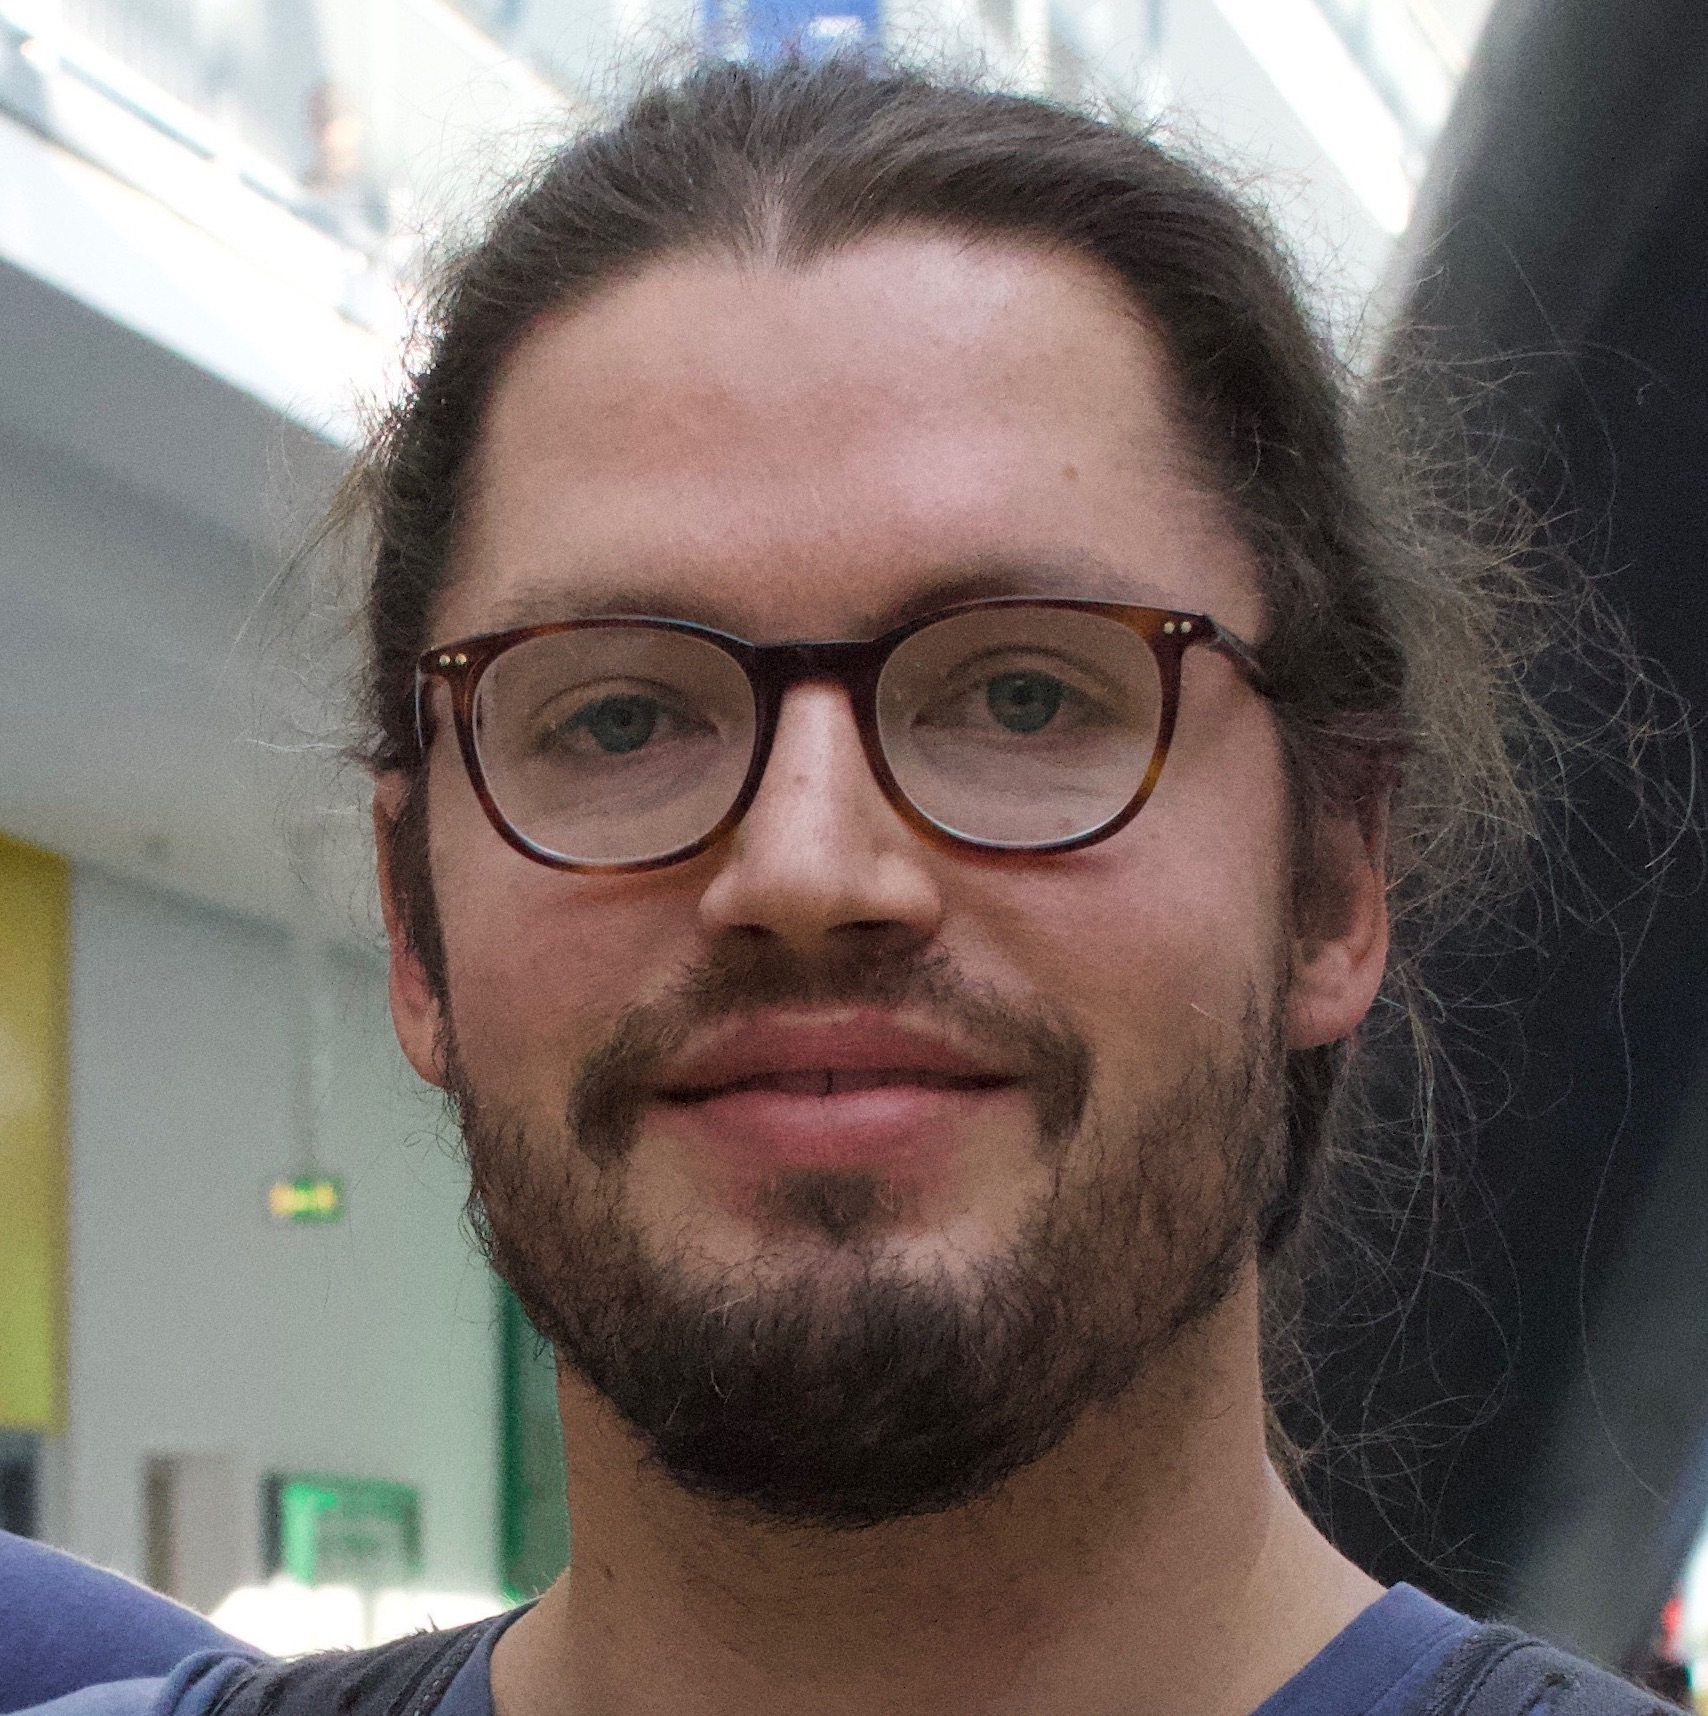
\includegraphics[height=1.5cm,width=1.5cm]{0-fig-people/jf2.jpg} \hspace{7em}%
  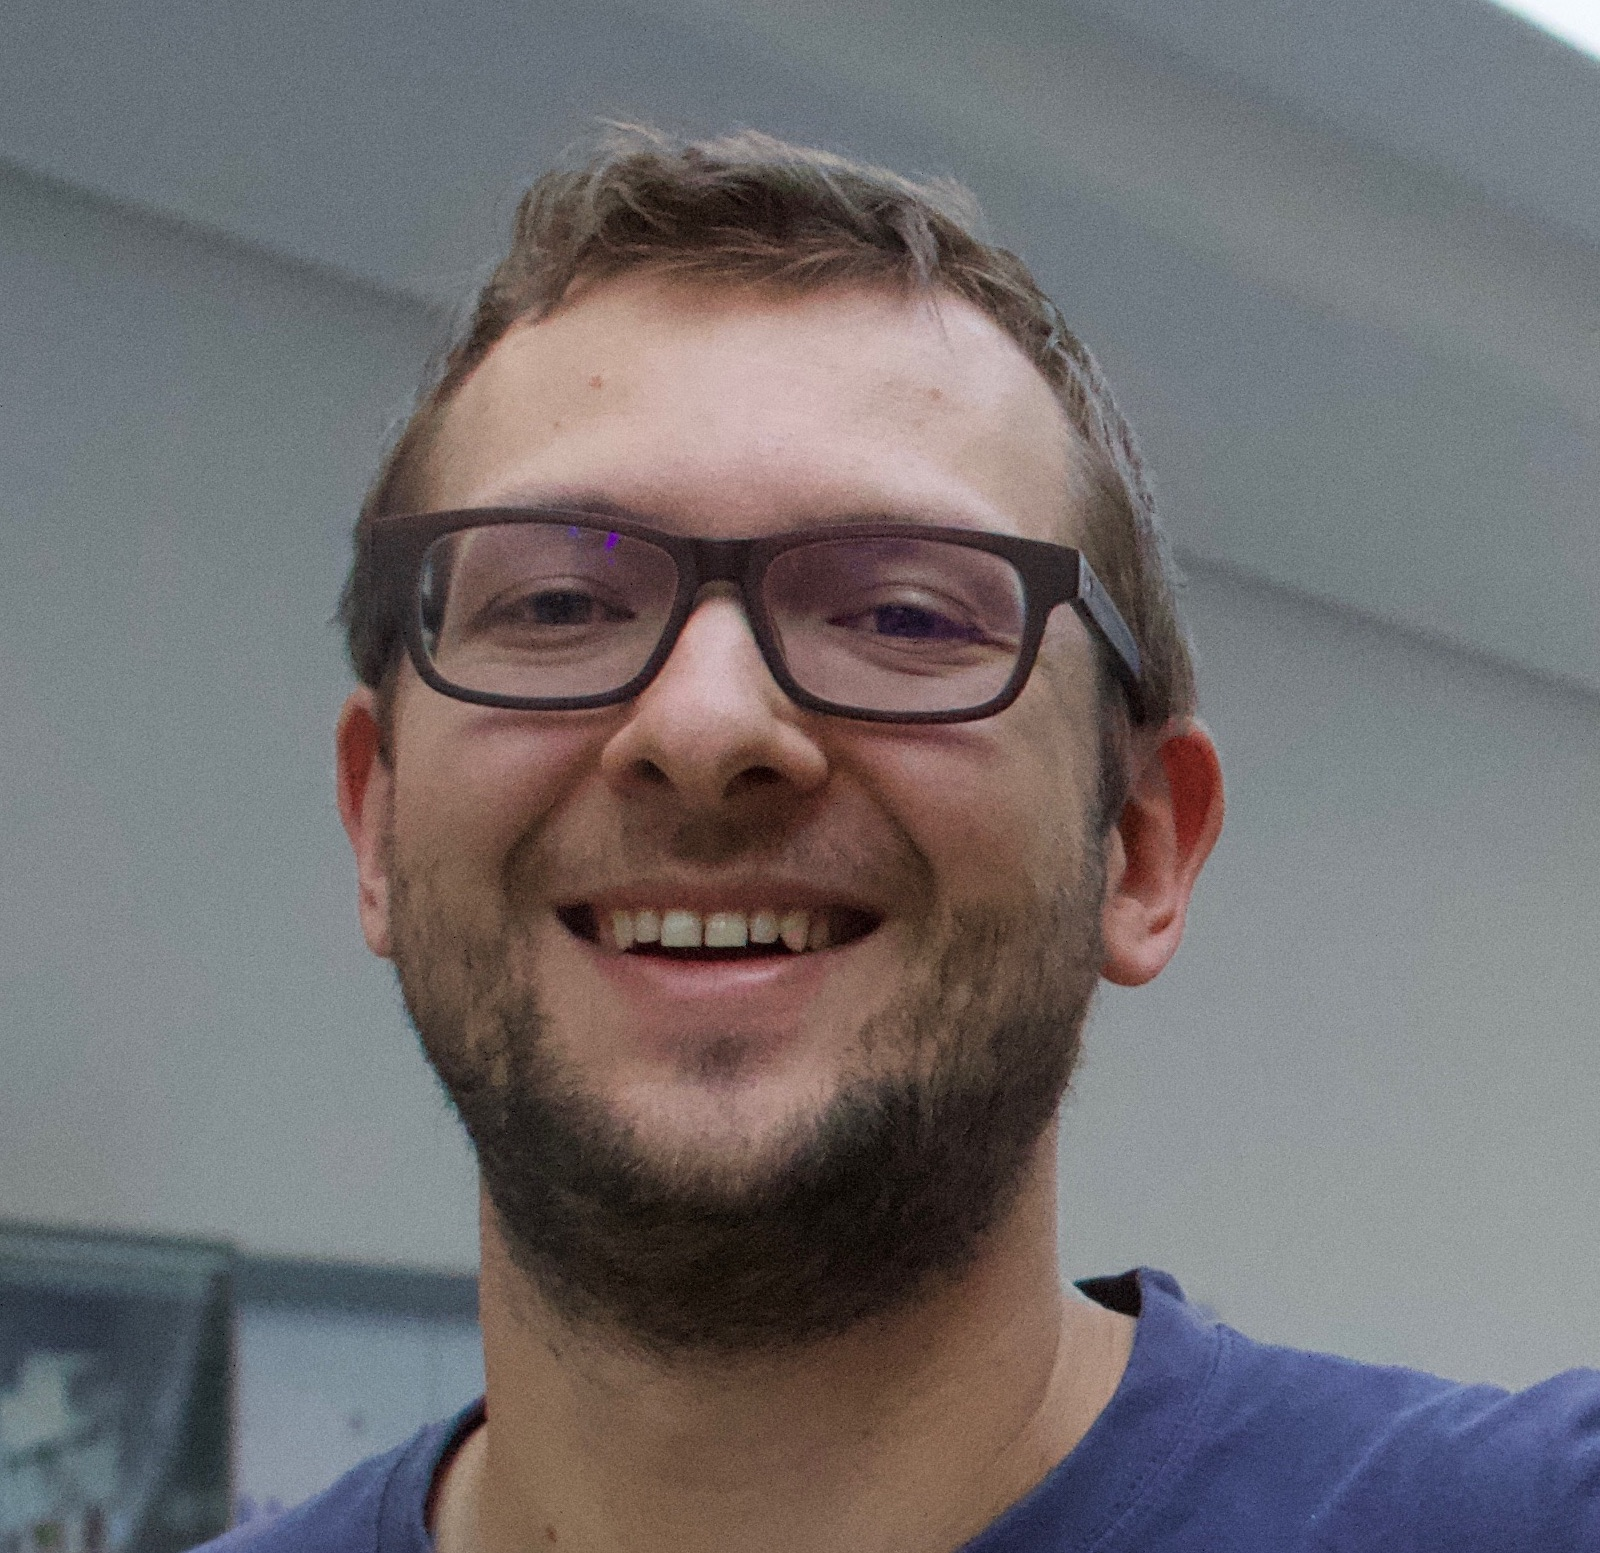
\includegraphics[height=1.5cm,width=1.5cm]{0-fig-people/mh2.jpg} \hspace{7em}%
  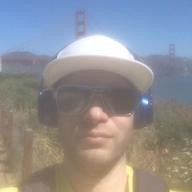
\includegraphics[height=1.5cm,width=1.5cm]{0-fig-people/pt.jpg} \hspace{7em}%
  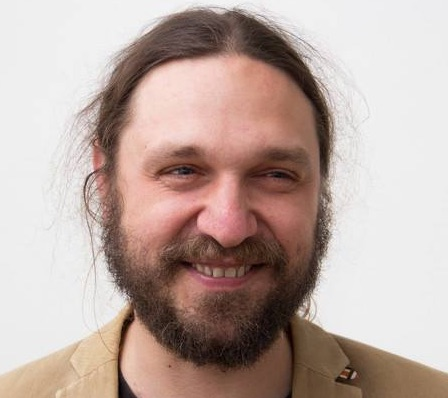
\includegraphics[height=1.5cm,width=1.7cm]{0-fig-people/sw2.jpg} \hspace{7em}%
  \\
  \vspace{0.5em}
  22nd International Symposium on Practical Aspects\\
  of Declarative Languages (PADL 2020)\\[1em]
  New Orleans, LA, USA January 21, 2020%
}%
\institute{%
  $^1$TU Dresden, Germany\\[0.5ex]
  $^2$TU Wien, Austria\\[0.5ex]
  \tiny{$^3${University of Potsdam, Germany}}\\[2em]
  % Grants Y698, W1255-N23, P-26696\\[2.5em]%
  % %\tiny{$^3${Johannes Kepler University Linz, Austria}}%
  % %\\[2.5em]%\\[-0.2em]%
  % 
}

\usepackage{mytikz}
\newcommand{\pgftextsize}{\scriptsize}

\newcommand{\unchecked}{{\Large\makebox[0pt][l]{\phantom{$\square$}}\raisebox{.15ex}{\hspace{0.1em}}}}
\newcommand{\checked}{{\Large\makebox[0pt][l]{\phantom{$\square$}}\raisebox{.1ex}{\hspace{0.1em}$\checkmark$}}}

\usepackage{hanging}
\begin{document}
\loadpresentation{0-figs/graph0/td1.tex}
\loadpresentation{0-figs/graph0/td2.tex}



\section{Introduction}


\setcounter{framenumber}{0}
\maketitle


\begin{frame}{Motivation}
  \vspace{-1em}
  \begin{block}{Domain}
    \begin{itemize}
    \item Hard problems tractable when certain properties present
    \item Examples: Vertex Cover, Model Counting (\#SAT), ...
    \item \alert{Bounded treewidth} often leads to tractability in theory,
      e.g., problems expressible in monadic second-order logic (MSO)
    \end{itemize}
  \end{block}
  \vspace{-1em}
  \begin{block}{Approaches \uncover<2>{({\color{blue}Advantages}/{\color{red}Disadvantages})}:}
    \begin{enumerate}
    \item Design dynamic programming algorithm (DP) and implement it
    \item[\hspace{2em}\cmark]<2-> {\color{blue}Can perform well (e.g., gpusat \bcite{FHWZisser'18})}
    \item[\hspace{2em}\xmark\hspace{0.25em}]<2-> {\color{red}Pretty annoying to implement}
    \item Use MSO solver together with an MSO specification 
    \item[\hspace{2em}\xmark\hspace{0.25em}]<2-> {\color{red}Does not perform (e.g., Sequoia \bcite{Kneis\&Langer\&Rossmanith'11})}
    \item[\hspace{2em}\cmark]<2-> {\color{blue}Easy to implement and many theoretical descriptions available}
    \end{enumerate}
  \end{block}
\end{frame}


\begin{frame}{Research Question \uncover<2>{\& Approach}}
  \medskip
  \alert{Can we merge the two approaches? (and make it reasonable to use?)}\\[0.5em]
  \begin{itemize}
  \item[Idea 1:] Provide a programming framework.\\
    Already done.\\
    $\Rightarrow$ Sharp (C++) \bcite{Morak'11} and Jatatosk (Java) \bcite{Bannach\&Berndt'18}\\
    \hspace{1em}\xmark~still hard to use \hspace{4.7em} \xmark~performs nice, but far from competitive
    \medskip
  \item[Idea 2:] Use a logic based language to specify the DP\\
    Already done.\\
    $\Rightarrow$ D-FLAT (use ASP for spec and take an ASP solver for
    computation) \bcite{Bliem\&Morak\&Stefan Woltran'12}\\
    \hspace{1em}\xmark~still fairly hard to use and performs mostly not very well
    \color{red}
  \end{itemize}
  \uncover<2->{%
    
    \begin{itemize}
    \item[\color{red}Our idea:]<2-> \color{red}Use SQL to describe the
      DP and use a DB to evaluate the queries
    \end{itemize}
  }
\end{frame}

\begin{frame}{Outline}
\bigskip\bigskip\bigskip
  \begin{enumerate}
  \item Basics: Tree Decompositions\medskip
  \item Dynamic Programming Example and Computation for Model Counting
    (\#SAT)\medskip
  \item Our tool \texttt{dpdb}
  \end{enumerate}
\end{frame}

\subsection{Preliminaries}
\begin{frame}<1,2,10>[noframenumbering]{Tree Decompositions}\label{lbl:motivation}
  \only<1>{
  \bigskip
  \begin{columns}
    \begin{column}{0.5\textwidth}
      {\includegraphics[scale=0.15]{0-figs/tw}}
    \end{column}
    \begin{column}{0.5\textwidth}
      \includegraphics[scale=0.18]{0-figs/treedecomp}
    \end{column}
  \end{columns}    
  }%
  \only<2->{%
    \begin{center}
      \vspace{-2em}
      \begin{columns}
        \begin{column}{0.3\textwidth}
          \input{0-figs/graph0/graph2_m}
        \end{column}
        \begin{column}{0.3\textwidth}
          \uncover<10->{%
            \input{0-figs/graph0/td}
            %
          }%
        \end{column}
      \end{columns}
      \vspace{-3em}
    \end{center}
    % 
  }%

  \only<1>{%

  \begin{block}{Treewidth \hyperlink{treewidth}{\beamergotobutton{Definition \& Example}}}
    %\vspace{-0.5em}
    \begin{itemize}\itemsep5pt
    \item<1> Most prominent graph invariant 
    \item<1> Small treewidth indicates tree-likeness and sparsity
    \item<1> Can be used to solve \#SAT/WMC by defining graph\\
      representations of the input formula
    \end{itemize}
  \end{block}
  }%
  \only<2,10>{%
    \begin{block}{Treewidth \hyperlink{treewidth}{\beamergotobutton{Definition \& Example}}}
      % \vspace{-0.5em}
      \begin{itemize}\itemsep5pt
      \item Treewidth defined in terms of tree decompositions (TD)
      \item TD: arrangement of graph into a tree of bags s.t. ...
      \item<10> Treewidth: width of a TD of smallest width
      \end{itemize}
    \end{block}
  }%
\end{frame}

% \section{Tree Decompositions}
% \begin{frame}{``Treewidth''?}
%   \begin{columns}
%     \column{.05\textwidth}
%     \column{.65\textwidth}
%     {\includegraphics[scale=0.2]{0-figs/tw.jpg}}
%   \end{columns}
%   \begin{itemize}
%     \medskip
%   \item Many problems are (comput.) hard on graphs, but simpler on trees
%     \medskip
%   \item There is a way to capture how \alert{``tree-like''} a graph is -- the
%     treewidth, defined in terms of
%     \alert{tree decompositions} $\dots$
%     % 
%   \end{itemize}
% \end{frame}


%,label=td
\begin{frame}<10>[label=td]{Tree Decompositions}
  \begin{columns}[T]
    \begin{column}{.463\textwidth}
      \includegraphics[scale=0.21]{0-figs/treedecomp.jpg}
    \end{column}
    \begin{column}{.48\textwidth}
      \vspace{-1em}
      \begin{exampleblock}{Tree Decomposition $\mathcal{T}$ of $G$}
        \vspace{-1em}
        \begin{columns}
          \begin{column}{0.5\textwidth}
            \centering ~\hspace{1em}\input{0-figs/graph0/graph2_m}
          \end{column}
          \begin{column}{0.5\textwidth}
            \input{0-figs/graph0/td}\\[1em]
          \end{column}
        \end{columns}
      \end{exampleblock}
    \end{column}
  \end{columns}
  \vspace{-2.5ex}
  \begin{block}{Definition}
    % \hyperlink{tw_basics<1>}{\beamergotobutton{Formally}}}
    A tree decomposition is a tree obtained from an arbitrary graph
    s.t.\
    \begin{enumerate}
    \item \textcolor<2>{red}{Each vertex} must occur in some
      \emph{bag}
    \item For \textcolor<3-7>{red}{each edge}, there is a bag
      containing both endpoints
    \item %\emph{Connectedness condition}:\\
      \textcolor<8-9>{red}{\emph{Connected}}: Tree ``restricted'' to any vertex must be connected
    \end{enumerate}
  \end{block}
\end{frame}




\begin{frame}[noframenumbering]{}
  \bigskip
  \bigskip
  \bigskip
  \bigskip
  \bigskip
  \bigskip
  \begin{center}
    \alert{\Large ``Find'' tree decompositions of small width?}\\

    \bigskip

    \uncover<2>{%
      Works well even for relatively large instances.\\[1em]
      Thanks to the Parameterized Algorithms and\\
      Computational Experiments Challenge \\
      (PACE) '16/'17!!!
      %
    }

  \end{center}
\end{frame}


\begin{frame}[noframenumbering]{}
  \bigskip
  \bigskip
  \bigskip
  \bigskip
  \bigskip
  \bigskip
  \begin{center}
    \alert{\Large How to ``use'' tree decompositions for \#SAT/WMC?}\\
  \end{center}
\end{frame}

\begin{frame}{Approach / Dynamic Programming}
  \bigskip\bigskip\bigskip
  \centering
  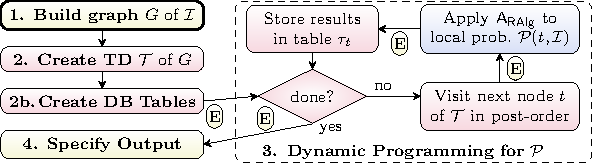
\includegraphics[scale=1.2]{0-figs/figure}
\end{frame}


\begin{frame}<1-5,11,16>[label=sat]{Example Problem of Interest}
  \medskip
  \begin{block}{SAT-Problem (Boolean Satisfiability Problem)}
    \begin{tabular}[t]{ll}
      Given: & Propositional formula $F$.\\
      Question: & Is there a truth assignment~$\tau$ to the variables\\
             & in $F$ such that $F_\tau$ evaluates to $1$ (\emph{satisfiable}).
    \end{tabular}\\
    %\hfill\hyperlink{sat<16>}{\beamergotobutton{Skip Example}}
  \end{block}
  \vspace{-1.2em}
  \only<1-2>{
  \uncover<2->{
  \begin{block}{Input normal form}
    \begin{itemize}
    \item Conjunctive normal form (CNF)
    \item Form:
      $F = (\ell_1 \vee \ell_2 \vee \ell_3) \wedge \ldots \wedge
      (\ldots)$
 where $\ell_i$ either $x$ or $\neg x$
    \end{itemize}
  \end{block}
  }}
  \only<3->{
    \begin{block}{Example}
      % -1 -2 3 4 5 0
      \only<1-20>{%
        \vspace{-2em}
        \only<3>{%
          \vspace{0.5em}
          \begin{align*}
            F = ( \neg a \vee b \vee x) \wedge (a \vee b) \wedge (c \vee \neg x) \wedge (b \vee \neg c) \wedge (\neg b \vee \neg c \vee \neg y)
          \end{align*}
        } %
        \only<4>{%
          \begin{align*}
            F = ( \neg \vf{a} \vee \vt{b} \vee \vf{x}) \wedge 
            (\vf{a} \vee \vt{b}) \wedge (\vf{c} \vee \neg \vf{x}) 
            \wedge (\vt{b} \vee \neg \vf{c}) \wedge 
            (\neg \vt{b} \vee \neg \vf{c} \vee \neg \vf{y})
          \end{align*}
        }
        \only<5->{%
          \begin{align*}
            F = \cancelto{1}{( \neg \vf{a} \vee \vt{b} \vee \vf{x})} \wedge 
            \cancelto{1}{(\vf{a} \vee \vt{b})} \wedge 
            \cancelto{1}{(\vf{c} \vee \neg \vf{x})} 
            \cancelto{1}{\wedge (\vt{b} \vee \neg \vf{c})} \wedge 
            \cancelto{1}{(\neg \vt{b} \vee \neg \vf{c} \vee \neg \vf{y})}
          \end{align*}
        }
        \\[0.5em]
        \only<11->{%
          \begin{center}
            \alert{%
              $\Rightarrow$ Satisfiable\\[1em]
            }
          \end{center}
        }%  
      }%
    \end{block}
  }
  \uncover<16->{%
    \begin{block}{Model Counting (\#SAT/Number SAT)}
      \begin{itemize}
      \item Number of of satisfying truth assignments to~$F$.
      \end{itemize}
    \end{block}
    %
  }%
\end{frame}



\newcommand{\hsep}{\ensuremath{\leftarrow}}
\begin{frame}<-2>[label=solving]{Solving \#SAT \textcolor{blue}{[SamerSzeider10]}}
  \vspace{-0.5em}
  \begin{exampleblock}{$F=$\textcolor<4>{red}{$(\neg a \vee b
        \vee x)$} $\wedge$ \textcolor<4>{red}{$(a \vee b)$} $\wedge$
      \textcolor<5>{red}{$(c \vee \neg x)$} $\wedge$
      \textcolor<5-9>{red}{$(b \vee \neg c)$} $\wedge$
      \textcolor<7>{red}{$(\neg b \vee \neg c \vee \neg y)$}}
    \only<1>{
      \vspace{-1.5em}
      \begin{align*}
        \mathit{Mod}(F) & =\{ &
                                      \{b\},
                                      \{a,b\},
                                      \{b,c\}, 
                                      \{a,b,c\}, \\
                              &&
                                 \{b,c,x\},
                                 \{a,b,c,x\},\\
                              &&
                                 \{b,y\},
                                 \{a,b,y\}
                                 \}
      \end{align*}
      \vspace{-4em}
    }%
    %\uncover<3->{\include{0-figs/graphplus/graph_m_simple}}
    \begin{columns}[T]
      \begin{column}{.5\textwidth}
        %\vspace{-1em}
        \begin{enumerate}
        \item<2-> Create graph representation
        \item<3-> Decompose graph
        \item<4-> Solve subproblems
        \item<11-> Combine rows
      \end{enumerate}
      \uncover<3->{%
        \vspace{-1em}
        \begin{tikzpicture}[font=\small,baseline={(current bounding box.south)}]%
          \tikzset{ every node/.style={anchor=north} }%
          \node[] at (5.5,3.65) (nid) {};%
          \node[tdnode, label=right:{$ $}] at (5.5,2.9) (n8)
          {$b,\; c$};%
          \node <9> [color=red,tdnode,
          label=right:\textcolor{red}{$ $}] at (5.5,2.9) (n8)
          {$b,\; c$};%
          \node[tdnode, label=left:{$ $}] at (4.7,2.2) (n4)
          {$b,\; c$};%
          \node <6> [color=red,tdnode,
          label=left:\textcolor{red}{$ $}] at (4.7,2.2) (n4)
          {$b,\; \textcolor{red}{c}\textcolor{red}{}$};%
          \node [tdnode, label=left:{$ $}] at (4.7,1.5) (n10)
          {$b,\;x,\;c$};%
          \node <5> [color=red, tdnode,
          label=left:\textcolor{red}{$ $}] at (4.7,1.5) (n10)
          {$b,\;x,\;c$};%
          \node [tdnode, label={[xshift=0.4cm]left:{$\qquad\quad $}}]
          at (4.7,0.8) (n1) {$b,\; x,\; a$};%
          \node <4> [color=red, tdnode,
          label={[xshift=0.4cm]left:\textcolor{red}{$\qquad\quad $}}]
          at (4.7,0.8) (n1)
          {$\textcolor{red}{b,\; x,\; a}\textcolor{red}{}$};%
 
          \node[tdnode, label=above right:{$ $}] at (6.5,2.2) (n7)
          {$b,\; c$};%
          \node <8> [color=red,tdnode, label=above
          right:\textcolor{red}{$ $}] at (6.5,2.2) (n7) {$b,\; c$};%
          \node <8> [color=red,tdnode, label=above
          right:\textcolor{red}{$ $}] at (6.5,2.2) (n7)
          {$\textcolor{red}{b,\; c}$};%
          \node[tdnode, label=left:{$ $}] at (6.5,1.5) (n6)
          {$b,\;c,\;y$};%
          \node <7> [color=red,tdnode,
          label=left:\textcolor{red}{$ $}] at (6.5,1.5) (n6)
          {$b,\;c,\;y$};%
          \draw[tdedge] (n8) -- (n4) -- (n10) -- (n1);%
          \draw[tdedge] (n8) -- (n7) -- (n6);%
        \end{tikzpicture}%
      }%
      \\
      \vspace{1em}%
      \hspace{1em} \only<4->{%
        ``Local formula''~$F_t$ clauses whose\\ \hspace{1.2em} variables are
        contained in the bag\\ \hspace{1.5em}\uncover<4->{(colored in red above)}
        % 
      }
    \end{column}
    \begin{column}{.5\textwidth}
      \medskip
      \only<2>{%
        \vspace{2em}
        \resizebox{0.5\columnwidth}{!}{%
          {\color{blue}
        \begin{tikzpicture}[font=\small,baseline={(current bounding box.center)}]%
          \tikzset{ every node/.style={anchor=north} }%
          \node[](a){a};
          \node[left of=a](b){b};
          \node[below of=a](x){x};

          \node[left of=x](c){c};
          \node[left of=c](y){y};

          \draw[] (a) -- (b) -- (x) -- (a);%
          \draw[] (c) -- (x); %
          \draw[] (b) -- (c) -- (y) -- (b);%
        \end{tikzpicture}%        
        }%
        %
        }%
      }%
      \only<3>{%
        {~ %Determine origin row, copy values for current-bag and handle
        \begin{itemize}
        \item[LEAF.:] Put empty set and counter 1
        \item[INTR.:]
          Guess truth value and check satisfiability 
          %\begin{itemize} 
% ($a \mapsto 0$ or $a \mapsto 1$)
%           \item Consider $\tau_a = \tau \cup \{a \mapsto 1\}$ and
%             $\tau_{\neg a} = \tau \cup \{a \mapsto 0\}$\\
%             (old assignment with(out) a)
%           \item Check satisfiability\\
%             ($\tau_a \models F_t$? $\tau_{\neg a} \models F_t$?)
          %\end{itemize}
          % \item[INTR. clause:] Mark if satisfied
        \item[REMOVE:] Remove $a$ from each assignment (row) in the
          table and sum up the counters if we get multiple assignments
          with the same data
        %\item[REM. clause:] Check satisfiability
        \item[JOIN:] Match rows with the same assignment and multiply
          the counters
        %\item[JOIN clause:] Mark if satisfied in some origin row
        \end{itemize} 
        % \begin{itemize}
        % \item[INTR. atom:] Guess truth-value, mark sat. clauses
        % \item[INTR. clause:] Mark if satisfied
        % \item[REMOVE atom:] Nothing to do
        % \item[REM. clause:] Check satisfiability
        % \item[JOIN atom:] Check truth-value agreement
        % \item[JOIN clause:] Mark if satisfied in some origin row
        % \end{itemize} 
        }
        % 
      }
      \only<4-11>{\def\highlightthings{\rowcolor<11> {HighlightColor}}
        \input{0-figs/graph0/ids-tables/tables_sat}}%
      \only<12->{\def\highlightthings{ }
        \input{0-figs/graph0/ids-tables/tables_ssat}}
      \vspace{1ex}
    \end{column}
  \end{columns}
  \end{exampleblock}
\end{frame}


%\section{Answer Set Programming}
%\newcommand{\hsep}{\ensuremath{\leftarrow}}
\begin{frame}<3->[]{Solving \#SAT \textcolor{blue}{[SamerSzeider'10]}}
  \vspace{-0.5em}
  \begin{exampleblock}{$F=$\textcolor<4>{red}{$(\neg a \vee b
        \vee x)$} $\wedge$ \textcolor<4>{red}{$(a \vee b)$} $\wedge$
      \textcolor<5>{red}{$(c \vee \neg x)$} $\wedge$
      \textcolor<5-9>{red}{$(b \vee \neg c)$} $\wedge$
      \textcolor<7>{red}{$(\neg b \vee \neg c \vee \neg y)$}}
    \only<1>{
      \vspace{-1.5em}
      \begin{align*}
        \mathit{Mod}(F) & =\{ &
                                      \{b\},
                                      \{a,b\},
                                      \{b,c\}, 
                                      \{a,b,c\}, \\
                              &&
                                 \{b,c,x\},
                                 \{a,b,c,x\},\\
                              &&
                                 \{b,y\},
                                 \{a,b,y\}
                                 \}
      \end{align*}
      \vspace{-4em}
    }%
    %\uncover<3->{\include{0-figs/graphplus/graph_m_simple}}
    \begin{columns}[T]
      \begin{column}{.5\textwidth}
        %\vspace{-1em}
        \begin{enumerate}
        \item<2-> Create graph representation
        \item<3-> Decompose graph
        \item<4-> Solve subproblems
        \item<11-> Combine rows
      \end{enumerate}
      \uncover<3->{%
        \vspace{-1em}
        \begin{tikzpicture}[font=\small,baseline={(current bounding box.south)}]%
          \tikzset{ every node/.style={anchor=north} }%
          \node[] at (5.5,3.65) (nid) {};%
          \node[tdnode, label=right:{$ $}] at (5.5,2.9) (n8)
          {$b,\; c$};%
          \node <9> [color=red,tdnode,
          label=right:\textcolor{red}{$ $}] at (5.5,2.9) (n8)
          {$b,\; c$};%
          \node[tdnode, label=left:{$ $}] at (4.7,2.2) (n4)
          {$b,\; c$};%
          \node <6> [color=red,tdnode,
          label=left:\textcolor{red}{$ $}] at (4.7,2.2) (n4)
          {$b,\; \textcolor{red}{c}\textcolor{red}{}$};%
          \node [tdnode, label=left:{$ $}] at (4.7,1.5) (n10)
          {$b,\;x,\;c$};%
          \node <5> [color=red, tdnode,
          label=left:\textcolor{red}{$ $}] at (4.7,1.5) (n10)
          {$b,\;x,\;c$};%
          \node [tdnode, label={[xshift=0.4cm]left:{$\qquad\quad $}}]
          at (4.7,0.8) (n1) {$b,\; x,\; a$};%
          \node <4> [color=red, tdnode,
          label={[xshift=0.4cm]left:\textcolor{red}{$\qquad\quad $}}]
          at (4.7,0.8) (n1)
          {$\textcolor{red}{b,\; x,\; a}\textcolor{red}{}$};%
 
          \node[tdnode, label=above right:{$ $}] at (6.5,2.2) (n7)
          {$b,\; c$};%
          \node <8> [color=red,tdnode, label=above
          right:\textcolor{red}{$ $}] at (6.5,2.2) (n7) {$b,\; c$};%
          \node <8> [color=red,tdnode, label=above
          right:\textcolor{red}{$ $}] at (6.5,2.2) (n7)
          {$\textcolor{red}{b,\; c}$};%
          \node[tdnode, label=left:{$ $}] at (6.5,1.5) (n6)
          {$b,\;c,\;y$};%
          \node <7> [color=red,tdnode,
          label=left:\textcolor{red}{$ $}] at (6.5,1.5) (n6)
          {$b,\;c,\;y$};%
          \draw[tdedge] (n8) -- (n4) -- (n10) -- (n1);%
          \draw[tdedge] (n8) -- (n7) -- (n6);%
        \end{tikzpicture}%
      }%
      \\
      \vspace{1em}%
      \hspace{1em} \only<4>{%
        ``Local formula''~$F_t$ clauses whose\\ \hspace{1.2em} variables are
        contained in the bag\\ \hspace{1.5em}\uncover<4>{(colored in red above)}
        % 
      }
    \end{column}
    \begin{column}{.5\textwidth}
      \medskip
      \only<2>{%
        \vspace{2em}
        \resizebox{0.5\columnwidth}{!}{%
          {\color{blue}
        \begin{tikzpicture}[font=\small,baseline={(current bounding box.center)}]%
          \tikzset{ every node/.style={anchor=north} }%
          \node[](a){a};
          \node[left of=a](b){b};
          \node[below of=a](x){x};

          \node[left of=x](c){c};
          \node[left of=c](y){y};

          \draw[] (a) -- (b) -- (x) -- (a);%
          \draw[] (c) -- (x); %
          \draw[] (b) -- (c) -- (y) -- (b);%
        \end{tikzpicture}%        
        }%
        %
        }%
      }%
      \only<4-11>{\def\highlightthings{\rowcolor<11> {HighlightColor}}
        \input{0-figs/graph0/ids-tables/tables_sat}}%
      \only<12->{\def\highlightthings{ }
        \input{0-figs/graph0/ids-tables/tables_ssat}}
      \vspace{1ex}
    \end{column}
  \end{columns}
  \end{exampleblock}
\end{frame}


% \begin{frame}<3>[label=current]{Solving \#SAT \textcolor{blue}{[SamerSzeider'10]}}
%   \vspace{-0.5em}
%   \begin{exampleblock}{$F=$\textcolor<4>{red}{$(\neg a \vee b
%         \vee x)$} $\wedge$ \textcolor<4>{red}{$(a \vee b)$} $\wedge$
%       \textcolor<5>{red}{$(c \vee \neg x)$} $\wedge$
%       \textcolor<5-9>{red}{$(b \vee \neg c)$} $\wedge$
%       \textcolor<7>{red}{$(\neg b \vee \neg c \vee \neg y)$}}
%     \only<1>{
%       \vspace{-1.5em}
%       \begin{align*}
%         \mathit{Mod}(F) & =\{ &
%                                       \{b\},
%                                       \{a,b\},
%                                       \{b,c\}, 
%                                       \{a,b,c\}, \\
%                               &&
%                                  \{b,c,x\},
%                                  \{a,b,c,x\},\\
%                               &&
%                                  \{b,y\},
%                                  \{a,b,y\}
%                                  \}
%       \end{align*}
%       \vspace{-4em}
%     }%
%     %\uncover<3->{\include{0-figs/graphplus/graph_m_simple}}
%     \begin{columns}[T]
%       \begin{column}{.5\textwidth}
%         %\vspace{-1em}
%         \begin{enumerate}
%         \item<2-> Create graph representation
%         \item<3-> Decompose graph
%         \item<4-> Solve subproblems
%         \item<11-> Combine rows
%       \end{enumerate}
%       \uncover<3->{%
%         \vspace{-1em}
%         \begin{tikzpicture}[font=\small,baseline={(current bounding box.south)}]%
%           \tikzset{ every node/.style={anchor=north} }%
%           \node[] at (5.5,3.65) (nid) {};%
%           \node[tdnode, label=right:{$ $}] at (5.5,2.9) (n8)
%           {$b,\; c$};%
%           \node <9> [color=red,tdnode,
%           label=right:\textcolor{red}{$ $}] at (5.5,2.9) (n8)
%           {$b,\; c$};%
%           \node[tdnode, label=left:{$ $}] at (4.7,2.2) (n4)
%           {$b,\; c$};%
%           \node <6> [color=red,tdnode,
%           label=left:\textcolor{red}{$ $}] at (4.7,2.2) (n4)
%           {$b,\; \textcolor{red}{c}\textcolor{red}{}$};%
%           \node [tdnode, label=left:{$ $}] at (4.7,1.5) (n10)
%           {$b,\;x,\;c$};%
%           \node <5> [color=red, tdnode,
%           label=left:\textcolor{red}{$ $}] at (4.7,1.5) (n10)
%           {$b,\;x,\;c$};%
%           \node [tdnode, label={[xshift=0.4cm]left:{$\qquad\quad $}}]
%           at (4.7,0.8) (n1) {$b,\; x,\; a$};%
%           \node <4> [color=red, tdnode,
%           label={[xshift=0.4cm]left:\textcolor{red}{$\qquad\quad $}}]
%           at (4.7,0.8) (n1)
%           {$\textcolor{red}{b,\; x,\; a}\textcolor{red}{}$};%
 
%           \node[tdnode, label=above right:{$ $}] at (6.5,2.2) (n7)
%           {$b,\; c$};%
%           \node <8> [color=red,tdnode, label=above
%           right:\textcolor{red}{$ $}] at (6.5,2.2) (n7) {$b,\; c$};%
%           \node <8> [color=red,tdnode, label=above
%           right:\textcolor{red}{$ $}] at (6.5,2.2) (n7)
%           {$\textcolor{red}{b,\; c}$};%
%           \node[tdnode, label=left:{$ $}] at (6.5,1.5) (n6)
%           {$b,\;c,\;y$};%
%           \node <7> [color=red,tdnode,
%           label=left:\textcolor{red}{$ $}] at (6.5,1.5) (n6)
%           {$b,\;c,\;y$};%
%           \draw[tdedge] (n8) -- (n4) -- (n10) -- (n1);%
%           \draw[tdedge] (n8) -- (n7) -- (n6);%
%         \end{tikzpicture}%
%       }%
%       \\
%       \vspace{1em}%
%       \hspace{1em} \only<2->{%
%         ``Local formula''~$F_t$ clauses whose\\ \hspace{1.2em} variables are
%         contained in the bag\\ \hspace{1.5em}\uncover<3->{(colored in red above)}
%         % 
%       }
%     \end{column}
%     \begin{column}{.5\textwidth}
%       \medskip
%       \only<2>{%
%         \vspace{2em}
%         \resizebox{0.5\columnwidth}{!}{%
%           {\color{blue}
%         \begin{tikzpicture}[font=\small,baseline={(current bounding box.center)}]%
%           \tikzset{ every node/.style={anchor=north} }%
%           \node[](a){a};
%           \node[left of=a](b){b};
%           \node[below of=a](x){x};

%           \node[left of=x](c){c};
%           \node[left of=c](y){y};

%           \draw[] (a) -- (b) -- (x) -- (a);%
%           \draw[] (c) -- (x); %
%           \draw[] (b) -- (c) -- (y) -- (b);%
%         \end{tikzpicture}%        
%         }%
%         %
%         }%
%       }%
%       \only<3>{%
%         {~ %Determine origin row, copy values for current-bag and handle
%           Nice Tree Decompositions\\
%           (note example left is not nice)
%           \begin{itemize}
%           \item[LEAF.:] Put empty set and counter 1
%           \item[INTR.:]
%             Guess truth value and check satisfiability 
%           %\begin{itemize} 
% % ($a \mapsto 0$ or $a \mapsto 1$)
% %           \item Consider $\tau_a = \tau \cup \{a \mapsto 1\}$ and
% %             $\tau_{\neg a} = \tau \cup \{a \mapsto 0\}$\\
% %             (old assignment with(out) a)
% %           \item Check satisfiability\\
% %             ($\tau_a \models F_t$? $\tau_{\neg a} \models F_t$?)
%           %\end{itemize}
%           % \item[INTR. clause:] Mark if satisfied
%         \item[REMOVE:] Remove $a$ from each assignment (row) in the
%           table and sum up the counters if we get multiple assignments
%           with the same data
%         %\item[REM. clause:] Check satisfiability
%         \item[JOIN:] Match rows with the same assignment and multiply
%           the counters
%         %\item[JOIN clause:] Mark if satisfied in some origin row
%         \end{itemize} 
%         % \begin{itemize}
%         % \item[INTR. atom:] Guess truth-value, mark sat. clauses
%         % \item[INTR. clause:] Mark if satisfied
%         % \item[REMOVE atom:] Nothing to do
%         % \item[REM. clause:] Check satisfiability
%         % \item[JOIN atom:] Check truth-value agreement
%         % \item[JOIN clause:] Mark if satisfied in some origin row
%         % \end{itemize} 
%         }
%         % 
%       }
%       \only<4-11>{\def\highlightthings{\rowcolor<11> {HighlightColor}}
%         \input{0-figs/graph0/ids-tables/tables_sat}}%
%       \only<12->{\def\highlightthings{ }
%         \input{0-figs/graph0/ids-tables/tables_ssat}}
%       \vspace{1ex}
%     \end{column}
%   \end{columns}
%   \end{exampleblock}
% \end{frame}

\begin{frame}<3>[label=current]{Solving \#SAT \textcolor{blue}{[SamerSzeider'10]}}
  \vspace{-0.5em}
  \begin{exampleblock}{$F=$\textcolor<4>{red}{$(\neg a \vee b
        \vee x)$} $\wedge$ \textcolor<4>{red}{$(a \vee b)$} $\wedge$
      \textcolor<5>{red}{$(c \vee \neg x)$} $\wedge$
      \textcolor<5-9>{red}{$(b \vee \neg c)$} $\wedge$
      \textcolor<7>{red}{$(\neg b \vee \neg c \vee \neg y)$}}
    \only<1>{
      \vspace{-1.5em}
      \begin{align*}
        \mathit{Mod}(F) & =\{ &
                                      \{b\},
                                      \{a,b\},
                                      \{b,c\}, 
                                      \{a,b,c\}, \\
                              &&
                                 \{b,c,x\},
                                 \{a,b,c,x\},\\
                              &&
                                 \{b,y\},
                                 \{a,b,y\}
                                 \}
      \end{align*}
      \vspace{-4em}
    }%
    %\uncover<3->{\include{0-figs/graphplus/graph_m_simple}}
    \begin{columns}[T]
      \begin{column}{.5\textwidth}
        %\vspace{-1em}
        \begin{enumerate}
        \item<2-> Create graph representation
        \item<3-> Decompose graph
        \item<4-> Solve subproblems
        \item<11-> Combine rows
      \end{enumerate}
      \uncover<3->{%
        \vspace{-1em}
        \begin{tikzpicture}[font=\small,baseline={(current bounding box.south)}]%
          \tikzset{ every node/.style={anchor=north} }%
          \node[] at (5.5,3.65) (nid) {};%
          \node[tdnode, label=right:{$ $}] at (5.5,2.9) (n8)
          {$b,\; c$};%
          \node <9> [color=red,tdnode,
          label=right:\textcolor{red}{$ $}] at (5.5,2.9) (n8)
          {$b,\; c$};%
          \node[tdnode, label=left:{$ $}] at (4.7,2.2) (n4)
          {$b,\; c$};%
          \node <6> [color=red,tdnode,
          label=left:\textcolor{red}{$ $}] at (4.7,2.2) (n4)
          {$b,\; \textcolor{red}{c}\textcolor{red}{}$};%
          \node [tdnode, label=left:{$ $}] at (4.7,1.5) (n10)
          {$b,\;x,\;c$};%
          \node <5> [color=red, tdnode,
          label=left:\textcolor{red}{$ $}] at (4.7,1.5) (n10)
          {$b,\;x,\;c$};%
          \node [tdnode, label={[xshift=0.4cm]left:{$\qquad\quad $}}]
          at (4.7,0.8) (n1) {$b,\; x,\; a$};%
          \node <4> [color=red, tdnode,
          label={[xshift=0.4cm]left:\textcolor{red}{$\qquad\quad $}}]
          at (4.7,0.8) (n1)
          {$\textcolor{red}{b,\; x,\; a}\textcolor{red}{}$};%
 
          \node[tdnode, label=above right:{$ $}] at (6.5,2.2) (n7)
          {$b,\; c$};%
          \node <8> [color=red,tdnode, label=above
          right:\textcolor{red}{$ $}] at (6.5,2.2) (n7) {$b,\; c$};%
          \node <8> [color=red,tdnode, label=above
          right:\textcolor{red}{$ $}] at (6.5,2.2) (n7)
          {$\textcolor{red}{b,\; c}$};%
          \node[tdnode, label=left:{$ $}] at (6.5,1.5) (n6)
          {$b,\;c,\;y$};%
          \node <7> [color=red,tdnode,
          label=left:\textcolor{red}{$ $}] at (6.5,1.5) (n6)
          {$b,\;c,\;y$};%
          \draw[tdedge] (n8) -- (n4) -- (n10) -- (n1);%
          \draw[tdedge] (n8) -- (n7) -- (n6);%
        \end{tikzpicture}%
      }%
      \\
      \vspace{1em}%
      \hspace{1em} \only<2->{%
        ``Local formula''~$F_t$ clauses whose\\ \hspace{1.2em} variables are
        contained in the bag\\ \hspace{1.5em}\uncover<3->{(colored in red above)}
        % 
      }
    \end{column}
    \begin{column}{.5\textwidth}
      \medskip
      \only<2>{%
        \vspace{2em}
        \resizebox{0.5\columnwidth}{!}{%
          {\color{blue}
        \begin{tikzpicture}[font=\small,baseline={(current bounding box.center)}]%
          \tikzset{ every node/.style={anchor=north} }%
          \node[](a){a};
          \node[left of=a](b){b};
          \node[below of=a](x){x};

          \node[left of=x](c){c};
          \node[left of=c](y){y};

          \draw[] (a) -- (b) -- (x) -- (a);%
          \draw[] (c) -- (x); %
          \draw[] (b) -- (c) -- (y) -- (b);%
        \end{tikzpicture}%        
        }%
        %
        }%
      }%
      \only<3>{%
        \resizebox{.6\linewidth}{!}{%
          \begin{algorithm}[H]
            % \centering
            \KwData{Variables~$V_t$ at $t$, previously computed
              tables~$T_{\downarrow{l}}$ and $T_{\downarrow{r}}$\\
              {~\bf Out:} New Table}
            % 
            \lIf(\hspace{-1em})
            % 
            {$\leaf$}{%
              \Return
              $ \left(\begin{matrix} cnt \\ \hline 1 \end{matrix}\right)$ 
              % 
            }%
            \uElseIf{$\intr$ and $a\in V_t$ new}{ %
              \Return $\sigma_{row \models F_t}\left(
                \overset{T_\downarrow}{\left(
                    \begin{matrix}
                      x_1 & x_2 & \ldots & cnt\\\hline
                      \ldots & \ldots & \ldots \\
                      \ldots & \ldots & \ldots \\
                    \end{matrix}
                  \right)} \bowtie \left(\begin{matrix} a \\\hline 0 \\
                    1 \end{matrix}\right)\right)$
            } %
            \uElseIf{$\rem$, and $a \not\in V_t$ removed}{%
              \Return 
              $\left( \begin{matrix}x_1 &  x_2 & a  & cnt &\\\hline 
                  % \vspace{-0.5em}
                  0 & 0 & 0 & \cancel{c^0_{00}} &
                  \hspace{-0.5em}\Rightarrow \sum_{c^0_{00}+c^1_{00}}\\
                  \rlap{\rule[0.6ex]{7em}{0.4pt}}0 & 0 & 1 & \cancel{c^1_{00}}\\
                  0 & 1 & 0 \makebox(-6,0){\rule[6ex]{0.4pt}{6\normalbaselineskip}}&
                  \cancel{c^1_{2}} &
                  \hspace{-0.5em}\Rightarrow \sum_{c^0_{01}+c^1_{01}}\\
                  \rlap{\rule[0.6ex]{7em}{0.4pt}}0 & 1 & 1 & \cancel{c^1_{2}}\\
                  \ldots
                \end{matrix}
              \right)$\\
              
            } %
            \uElseIf{$\join$}{%
                \Return $T_{\downarrow{}l} \bowtie
                T_{\downarrow{}r}$ +\\
                ``fix cnt (multiply from left and right)''
              % 
            } %
          \end{algorithm}%
          % 
        }%
        %
      }
      \only<4-11>{\def\highlightthings{\rowcolor<11> {HighlightColor}}
        \input{0-figs/graph0/ids-tables/tables_sat}}%
      \only<12->{\def\highlightthings{ }
        \input{0-figs/graph0/ids-tables/tables_ssat}}
      \vspace{1ex}
    \end{column}
  \end{columns}
  \end{exampleblock}
\end{frame}
\end{document}

\begin{frame}[label=current]{}
  \resizebox{.8\linewidth}{!}{%
\begin{algorithm}[H]
%\centering
  \KwData{Variables~$V_t$ at $t$, previously computed
    tables~$T_{\downarrow{l}}$ and $T_{\downarrow{r}}$\\
    {~\bf Out:} New Table}
  %
  \uIf(\hspace{-1em})
   %
  {$\leaf$}{%
    \Return
    $ \left(\begin{matrix} cnt \\ \hline 1 \end{matrix}\right)$ 
    %
  }%
  \uElseIf{$\intr$ and $a\in V_t$ new}{ %
    \Return $\sigma_{row \models F_t}\left(
      \overset{T_\downarrow}{\left(
      \begin{matrix}
        x_1 & x_2 & \ldots & cnt\\\hline
        \ldots & \ldots & \ldots \\
        \ldots & \ldots & \ldots \\
      \end{matrix}
    \right)} \bowtie \left(\begin{matrix} a \\\hline 0 \\
        1 \end{matrix}\right)\right)$
  } %
  \uElseIf{$\rem$, and $a \not\in V_t$ removed}{%
    \Return 
      \left( \begin{matrix}x_1 &  x_2 & a  & cnt &\\\hline 
        %\vspace{-0.5em}
        0 & 0 & 0 & \cancel{c^0_{00}} &
        \hspace{-0.5em}\Rightarrow \sum_{c^0_{00}+c^1_{00}}\\
        \rlap{\rule[0.6ex]{7em}{0.4pt}}0 & 0 & 1 & \cancel{c^1_{00}}\\
        0 & 1 & 0 \makebox(-6,0){\rule[6ex]{0.4pt}{6\normalbaselineskip}}&
        \cancel{c^1_{2}} &
        \hspace{-0.5em}\Rightarrow \sum_{c^0_{01}+c^1_{01}}\\
        \rlap{\rule[0.6ex]{7em}{0.4pt}}0 & 1 & 1 & \cancel{c^1_{2}}\\
        \ldots
        \end{matrix}
      \right)$\\
       % \makebox[-6,0]{\rule[1ex]{0.4pt}{3\normalbaselineskip}} 
     %
    } %
    \uElseIf{$\join$}{%
      \makebox[3.3cm][l]{%
        \Return $T_{\downarrow{}l} \bowtie
        T_{\downarrow{}r}$ + ``fix cnt (multiply from left and
        right)'' }
    % 
  } %
  % %\Return $\tab{t}$ \vspace{-0.25em}
  % % \caption{Alternative table algorithm~$\algo{S_{RAlg}}(t,\chi(t),\varphi_t,\langle \tab{1}, \ldots, \tab{\ell}\rangle)$ for \cSAT.}
  % % \label{alg:primdb}
\end{algorithm}%
%
}%
\end{frame}

\end{document}

\begin{frame}{Motivation}
  %\bigskip
  \begin{block}{Model Counting (\#SAT)}
    \begin{itemize}
    \item Generalizes Boolean satisfiability problem (SAT)
    \item \#SAT: output the number of satisfying assignments
    \item WMC: output the weighted model count
    % \item Low level language to encode combinatorial problems
    \item Various applications in AI and reasoning, e.g.,
      \begin{itemize}
      \item Bayesian reasoning \textcolor{blue}{[Sang et al.'05]}%~\cite{SangBeameKautz05a},
      \item Learning preference distributions \textcolor{blue}{[Choi et al.'15]}%~\cite{ChoiBroeckDarwiche15a},
      \item Infrastructure reliability \textcolor{blue}{[Meel et al.'17]} %~\cite{MeelEtAl17a}
      \end{itemize}
    \item Computational complexity: \#P-hard \textcolor{blue}{[Roth'96]} %~\cite{Roth96a}
    \end{itemize}
  \end{block}

  %\alert{Disclaimer: First part [ESA'18], second part unpublished}
\end{frame}

% \begin{frame}<1-11,16>[label=sat]{Problem of Interest}
%   \medskip
%   \begin{block}{SAT-Problem (Boolean Satisfiability Problem)}
%     \begin{tabular}[t]{ll}
%       Given: & Propositional formula $F$.\\
%       Question: & Is there a truth assignment~$\tau$ to the variables\\
%              & in $F$ such that $F_\tau$ evaluates to $1$ (\emph{satisfiable}).
%     \end{tabular}\\
%     \hfill\hyperlink{sat<16>}{\beamergotobutton{Skip Example}}
%   \end{block}
%   \vspace{-1.2em}
%   \only<1-2>{
%   \uncover<2->{
%   \begin{block}{Input normal form}
%     \begin{itemize}
%     \item Conjunctive normal form (CNF)
%     \item Form:
%       $F = (\ell_1 \vee \ell_2 \vee \ell_3) \wedge \ldots \wedge
%       (\ldots)$
%  where $\ell_i$ either $x$ or $\neg x$
%     \end{itemize}
%   \end{block}
%   }}
%   \only<3->{
%     \begin{block}{Example}
%       % -1 -2 3 4 5 0
%       \only<-11>{%
%         \vspace{-2em}
%         \only<3>{%
%           \vspace{0.5em}
%           \begin{align*}
%             (a \vee \neg b \vee d) \wedge (\neg a \vee \neg c \vee \neg d)
%             \wedge\\[1em]
%             (\neg a \vee \neg d) \wedge (b \vee c) \wedge (d \vee e )
%             \wedge (\neg b \vee \neg e)
%           \end{align*}
%         } \only<4->{%
%           \begin{align*}
%             \only<-3>{\\[-0.8em]}
%             \only<4>{\\[-1em]}
%             \only<4>{(\vf{a} \vee \neg \vf{b} \vee \vt{d})}
%             \only<5->{\cancelto{1}{(\vf{a} \vee \neg \vf{b} \vee \vt{d})}} 
%             \wedge
%             \only<-5>{(\neg \vf{a} \vee \neg \vt{c} \vee \neg \vt{d})}
%             \only<6->{\cancelto{1}{(\neg \vf{a} \vee \neg \vt{c} \vee \neg \vt{d})}}
%             \wedge
%             \only<-6>{\\[1em]}
%             \only<7->{\\[0.3em]}
%             \only<-6>{(\neg \vf{a} \vee \neg \vt{d})}
%             \only<7->{\cancelto{1}{(\neg \vf{a} \vee \neg \vt{d})}}
%             \wedge 
%             \only<-7>{(\vf{b} \vee \vt{c})}
%             \only<8->{\cancelto{1}{(\vf{b} \vee \vt{c})}}
%             \wedge 
%             \only<-8>{(\vt{d} \vee \vt{e})}
%             \only<9->{\cancelto{1}{(\vt{d} \vee \vt{e})}}
%             \wedge 
%             \only<-9>{(\neg \vf{b} \vee \neg \vt{e})}
%             \only<10-15>{\cancelto{1}{(\neg \vf{b} \vee \neg \vt{e})}}
%           \end{align*}
%         }
%         \\[0.5em]
%         \only<11->{%
%           \begin{center}
%             \alert{%
%               $\Rightarrow$ Satisfiable\\[1em]
%             }
%           \end{center}
%         }%  
%       }%
%       \only<12->{%
%         \vspace{-1.5em}
%         \only<-12>{%
%           \begin{align*}
%             (a \vee \neg b \vee d) \wedge 
%             (\neg a \vee \neg c \vee \neg d) \wedge \\[1em]
%             (\neg a \vee \neg d) \wedge 
%             (b \vee c) \wedge 
%             (d \vee e ) \wedge
%             (b \vee \neg e)% \wedge \\[1em]
%           \end{align*}
%         }%
%         \only<13->{%
%           \begin{align*}
%             (\vt{a} \vee \neg \vf{b} \vee \vf{d}) \wedge 
%             (\neg \vt{a} \vee \neg \vt{c} \vee \neg \vf{d})
%             \wedge
%             \only<13>{\\[0.8em]}
%             \only<14->{\\[0.2em]}
%             (\neg \vt{a} \vee \neg \vf{d}) \wedge 
%             (\vf{b} \vee \vt{c}) \wedge 
%             (\vf{d} \vee \vt{e} ) \wedge
%             \only<-13,16->{(\vf{b} \vee \vt{\neg e})}
%             \only<14-15>{\cancelto{0}{(\vf{b} \vee \vt{\neg e})}}
%             %\wedge \\[1em]
%           \end{align*}
%         }%
%         \uncover<15>{%
%           \vspace{-1.5em}
%           \begin{center}
%             \alert{%
%               $\Rightarrow$ Does not satisfy the formula.
%             }
%           \end{center}
%         }%
%       }
%     \end{block}
%   }
%   \vspace{-2em}
%   \uncover<16->{%
%     \begin{block}{\#SAT (Number SAT)}
%       \begin{itemize}
%       \item Number of of satisfying truth assignments to~$F$.
%       \end{itemize}
%     \end{block}
%     %
%   }%
% \end{frame}

% \begin{frame}<1>[label=sat]{The Problem of Interest}
%   \bigskip
%   \bigskip
%   % \begin{block}{SAT-Problem}
%   %   \begin{tabular}[t]{ll}
%   %     Given: & Propositional formula $F$.\\
%   %     Question: & Is there a truth assignment~$\tau$ to the variables\\
%   %            & in $F$ such that $F_\tau$ evaluates to $1$ (\emph{satisfiable}).
%   %   \end{tabular}
%   % \end{block}
%   \begin{block}{\#SAT (Number SAT)}
%     \begin{tabular}[t]{ll}
%       Given: & Propositional formula $F$.\\
%       Output: & Number of truth assignments~$\tau$ such that\\
%              & the formula~$F_\tau$ under the truth assignment\\
%              & evaluates to $1$ (\emph{satisfiable}).
%     \end{tabular}
%   \end{block}
% \end{frame}


% \begin{frame}{SAT Solver Evaluation}
% \centering
% \includegraphics[scale=0.75]{state_explosion_practice2}
% \end{frame}




% \begin{frame}{Problem of Interest cont.}
%   %\bigskip
%   \begin{block}{Weighted Model Counting (WMC)}
%     \begin{itemize}
%     \item Generalizes \#SAT
%     \item Given Boolean formula\uncover<2>{, e.g.,
%         $F=(x \vee y) \wedge (\neg x \vee \neg y)$}
%     \item[] Function that maps literals to reals between~$0$
%       and~$1$\uncover<2>{, e.g.,}
%     \item[]<2> $x \mapsto 0.4$, $\neg x \mapsto 0.6$, $y \mapsto 0.7$,
%       $\neg y \mapsto 0.3$
%     \item Weight of an assignment~$\alpha$ is the product over the
%       weights of its literals,~i.e.,
%       $w (\alpha) := \Pi_{v\in \alpha^{-1}(1)} w(v) \cdot \Pi_{v \in
%         \alpha^{-1}(0)} w(\neg v)$,
%     \item[]<2> e.g., $\alpha(x)=1$, $\alpha(y)=0$ $\Rightarrow$
%       $w(\alpha)=0.4 \cdot 0.3 = 0.16$
%     \item \emph{Weighted model count} (WMC) of formula is the sum of weights
%       over all its satisfying assignments% ,~i.e., %,~i.e.,
%       % $\Sigma_{\alpha \in 2^{\at(F)}, F(\alpha)=\emptyset}w(\alpha)$
%       \uncover<2>{, e.g.,}
%     \item[]<2> $w(F) = w(\alpha_1) + w(\alpha_2) = 0.12 + 0.42 = 0.54$
%     \end{itemize}
%   \end{block}
% \end{frame}


% \begin{frame}<1>[label=sat]{The Problem of Interest}
%   \bigskip
%   \bigskip
%   % \begin{block}{SAT-Problem}
%   %   \begin{tabular}[t]{ll}
%   %     Given: & Propositional formula $F$.\\
%   %     Question: & Is there a truth assignment~$\tau$ to the variables\\
%   %            & in $F$ such that $F_\tau$ evaluates to $1$ (\emph{satisfiable}).
%   %   \end{tabular}
%   % \end{block}
%   \begin{block}{\#SAT (Number SAT)}
%     \begin{tabular}[t]{ll}
%       Given: & Propositional formula $F$.\\
%       Output: & Number of truth assignments~$\tau$ such that\\
%              & the formula~$F_\tau$ under the truth assignment\\
%              & evaluates to $1$ (\emph{satisfiable}).
%     \end{tabular}
%   \end{block}
%   \medskip
%   \begin{block}{WMC (Number SAT)}
%     \begin{tabular}[t]{ll}
%       Given: & Propositional formula $F$.\\
%       Output: & Number of truth assignments~$\tau$ such that\\
%              & the formula~$F_\tau$ under the truth assignment\\
%              & evaluates to $1$ (\emph{satisfiable}).
%     \end{tabular}
%   \end{block}

% \end{frame}


% \begin{frame}{Motivation: What's the issue?}
%   \begin{columns}[t]
%     \begin{column}{0.8\textwidth}
%       \textbf{Theory:}\\
      
%       SAT cannot be solved faster than $2^{o(n)}$ steps!
%       (ETH)\\[2em]
      
%       % \centering
%       % \includegraphics[width=5.5cm]{universe.jpeg}
%       % $2^{280}$ $\mathbf{=}$ \# atoms in the universe\\
%       \uncover<2->{%
%         \textbf{Idea:}\\
%         \vspace{-1em}
%         \begin{columns}
%           \begin{column}{0.5\textwidth}
%             \begin{itemize}
%             \item Practical instances are usually highly structured
%             \item Structure can be exploited by algorithms
%             \end{itemize}
%           \end{column}
%           \begin{column}{0.5\textwidth}
%             \vspace{-3em}
%             \begin{figure}[!h]
%               \centering
%                 \resizebox{0.8\columnwidth}{!}{%
%                   \includegraphics[]{0-figs/longmult2}
%                 }%
%             \end{figure}
%           \end{column}
%         \end{columns}
%         %
%       }%
%     \end{column}
%   \end{columns}
%   \uncover<3->{%
%     \bigskip
%     \centering
%     \alert{\Ra Various Approaches in Solvers to exploit Structure}
%     % 
%   }%
% \end{frame}


\begin{frame}{Motivation: A somewhat different approach}
  \begin{block}{\#SAT/WMC Solving}
    \begin{itemize}
    \item There are already plenty solvers based on various techniques:\\
      approximate (Meel) / CDCL (Baccus/Thurley) /\\
      knowledge compilation based (Darwiche et al.)
    \end{itemize}
  \end{block}
  %
  \begin{block}{Parameterized Algorithms}
    \begin{itemize}
    \item Lots of theoretical work over last 20 years and various algorithms for \#SAT
    %\item There are various algorithms for \#SAT
    \end{itemize}
  \end{block}
  %
  \uncover<2->{%
    \begin{block}{Research Question}
      \alert{Are (theoretical) algorithms from parameterized complexity
        even useful for implementations in \#SAT/WMC solving?}
    \end{block}
    % 
  }
  % 
\end{frame}




% \begin{frame}{Motivation cont.}
%   \begin{block}{Can't we use techniques from SAT solvers?}
%     \begin{itemize}
%     \item Yes! see solvers\\
%       Cachet by F. Bacchus or\\
%       sharpSAT by M. Thurley
%     \item OR. sampling solutions by SAT solvers\\
%       approxMC by K. Meel
%     \item BUT: 
%     \end{itemize}
%   \end{block}
%   %
%   \uncover<2->{%
%     \begin{block}{Does it parallelize?}
%       \begin{itemize}
%       \item Not that I know of
%       \item Core techniques (CDCL) have inherent sequential properties [Sabharwal'14, Manthey'16]
%       \end{itemize}
%     \end{block}
%     % 
%   }
% \end{frame}



% \begin{frame}{Motivation cont.}
%   \begin{block}{Can't we use techniques from SAT solvers?}
%     \begin{itemize}
%     \item Yes! see solvers\\
%       Cachet by F. Bacchus or\\
%       sharpSAT by M. Thurley
%     \item OR. sampling solutions by SAT solvers\\
%       approxMC by K. Meel
%     \item BUT: 
%     \end{itemize}
%   \end{block}
%   %
%   \uncover<2->{%
%     \begin{block}{Does it parallelize?}
%       \begin{itemize}
%       \item Not that I know of
%       \item Core techniques (CDCL) have inherent sequential properties [Sabharwal'14, Manthey'16]
%       \end{itemize}
%     \end{block}
%     % 
%   }
% \end{frame}



% \begin{frame}{Motivation: What's the problem}
%   \bigskip\bigskip
%   \begin{columns}[t]
%     \begin{column}{0.5\textwidth}
%       \textbf{Theory:}\\
      
%       SAT cannot be solved faster than $2^{o(n)}$ steps!\\
%       (ETH: exponential time hypothesis)\\
      
%       % \centering
%       % \includegraphics[width=5.5cm]{universe.jpeg}
%       % $2^{280}$ $\mathbf{=}$ \# atoms in the universe\\
%     \end{column}
%     \begin{column}{0.5\textwidth}
%       \uncover<3>{%
%         \textbf{Practice:}\\
%         %\hspace{-2em}
%         \begin{itemize}
%         \item 1991(1st): $<215$ vars.
%         \item 2017: $>13\cdot 10^6$ vars (appl.)
%         \end{itemize}
%       }%
%     \end{column}
%   \end{columns}
  
%   \uncover<2->{%
%     \bigskip\bigskip
%     \centering
%     \alert{We still want to solve \#SAT!}
%     %
%   }

%   % \vspace{0.5cm}
%   % What is the reason for this huge discrepancy between theory and practice?
% \end{frame}



% \begin{frame}{Structure Matters!}
%   \begin{columns}
%     \begin{column}{0.5\textwidth}
%       \begin{itemize}
%       \item Classical complexity: only input size
%         taken into account
%       \item Practical instances are usually highly structured
%       \item Structure can be exploited by algorithms
%       \end{itemize}
%     \end{column}
%     \begin{column}{0.5\textwidth}
%       \begin{figure}[!h]
%         \centering
%         \includegraphics[scale=0.25]{longmult2}\\
%         %{\centering Industrial Instance\\
%         %  (multiplier verification)}
%       \end{figure}
%     \end{column}
%   \end{columns}
% \end{frame}


% \begin{frame}{What's structure for SAT solving?}
%   \bigskip
%   \begin{block}{Structure in Modern SAT Solvers}
%     \begin{itemize}
%     \item Many approaches: proof complexity... 
%     \item But honestly: we really don't know in theory!
%     \end{itemize}
%   \end{block}
% \end{frame}


\begin{frame}{Parameterized Algorithmics}
  \vspace{2em} %
  %\centering%
  %\Large
  \begin{alertblock}{Topic of the Talk}
    Solve \#SAT/WMC by means of an implementation of
    a  parameterized\\ algorithm that \alert{explicitly} \emph{exploits}
    small treewidth.
  \end{alertblock}
  \pause
  \vspace{1.5em}
  Presentation:
  \begin{enumerate}
  \item Ideas towards a GPU model counter \bcite{FHWoltranZ'18}
  \item Improved Architecture for \#SAT (this paper \bcite{FHZ'19})
  \end{enumerate}
  \vspace{1em}
  \pause
  Purpose:\\
  \alert{There are other architectures out there and it
    might fit for certain algorithms.\\
    NOT: outperforming everything else.}
\end{frame}


% \begin{frame}{Outline}
%   \bigskip\bigskip
%   \begin{enumerate}
%     % \item[0.] Motivation $\checked$% 
%   \item[1.] Motivation and the Problem (\#SAT) $\checked$% 
%   \item[2.] Treewidth of Formulas
%   \item[3.] 
%   \item[4.] Solving on the GPU
%   \end{enumerate}
% \end{frame}


% \begin{frame}[noframenumbering]{}
%   \bigskip
%   \bigskip
%   \bigskip
%   \bigskip
%   \bigskip
%   \bigskip
%   \begin{center}
%     \alert{\Large Basics: What is treewidth?}\\
%     \only<2>{%
%       \bigskip
%       Who knows about treewidth?
%       %
%     }
%   \end{center}
% \end{frame}


\subsection{Outline}

% \begin{frame}{Outline (Basic Architecture)}
%   \bigskip
%   %\centering
%   \begin{figure} \centering
%     \begin{tikzpicture}[      
%       every node/.style={anchor=south west,inner sep=0pt},
%       x=1mm, y=1mm,
%       ]   
%       \node (fig1) at (0,0)
%       {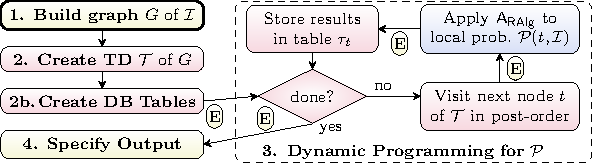
\includegraphics{0-figs/figure}};
%       %\node (fig2) at (3,3)
%       %{\includegraphics[scale=0.21]{example-image-b}};  
%     \end{tikzpicture}
%     %\caption{Using Tikz Overlay}
%   \end{figure}
%   Part:
%   \begin{enumerate}
%   \item[A)]<2-> Background \& Basic Concepts\\
%     {\footnotesize Treewidth, Graph Representation (1) + Dynamic Programming (3) [Samer \& Szeider JDA'10]}
%   \item[B)]<3-> Finding TDs (2)
%   \item[C)]<4-> Dynamic Programming (3) on the GPU
%   \end{enumerate}
% \end{frame}


\begin{frame}[noframenumbering]{}
  \bigskip
  \bigskip
  \bigskip
  \begin{center}
    \alert{\Large A GPU-based \#SAT/WMC-solver}\\[0.5em]
    OR how to go parallel?
  \end{center}
  \begin{columns}
    \begin{column}{0.3\textwidth}
      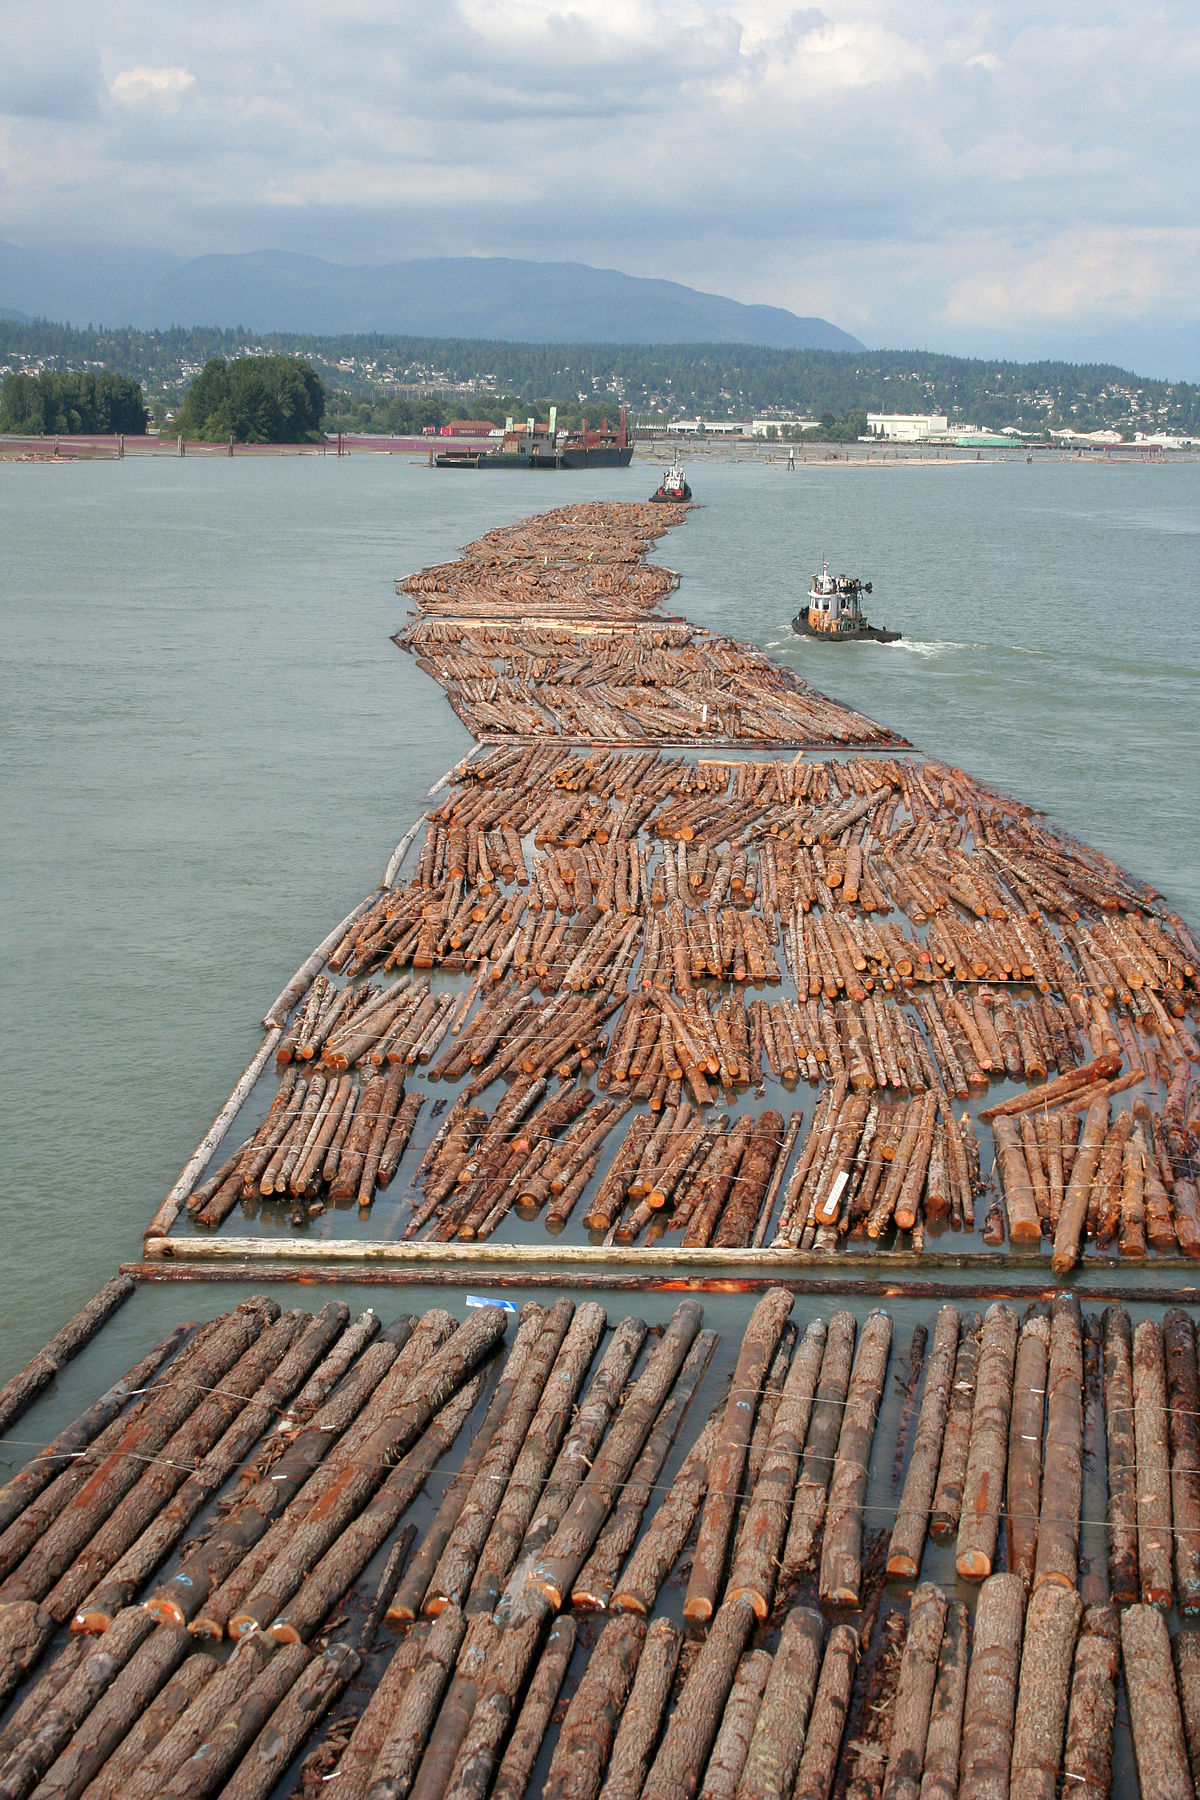
\includegraphics[scale=0.05]{0-figs/parallelization}
    \end{column}
    \hfill
    \begin{column}{0.3\textwidth}
      \includegraphics[scale=0.05]{0-figs/gpu_166}
      \vfill
    \end{column}
  \end{columns}
  % \includegraphics[scale=0.1]{fig/GPU_vs_CPU}

\end{frame}


\begin{frame}<1,15,16,17,18>{Dynamic Programming on the GPU}
  \begin{columns}
    \begin{column}{0.5\textwidth}
      \begin{block}{How to parallelize DP?}
        \begin{enumerate}
        \item<15-> Compute tables for multiple nodes in parallel
        \item<16->[\Ra] Does not allow for immediate massive
          parallelization due to dependencies to children
        \item<17-> Distribute computation of rows among different
          computation units
        \item<18->[\Ra] Allows with right hindsight for massive
          parallelization
        \item<18->[Why:] computation of rows are independent
        \end{enumerate}
      \end{block}
      \vfill
    \end{column}
    \begin{column}{0.5\textwidth}
      \only<1>{%
        \begin{figure}
          \includegraphics[scale=0.125]{0-figs/GPU_vs_CPU}
        \end{figure}
      }%
      % \only<2->{%
      %   \begin{figure}
      %     \includegraphics[scale=0.08]{fig/GPU_vs_CPU}
      %   \end{figure}
      % }%
      \uncover<4->{\def\highlightt{\rowcolor<17,18>{green}}\def\highlight{\rowcolor<17,18> {HighlightColor}}\def\highlightthings{}\input{0-figs/graph0/ids-tables/tables_simple_parallel}}
    \end{column}
  \end{columns}
\end{frame}



\begin{frame}<1>[noframenumbering]{Implementation}
  \only<1>{%
    \bigskip\bigskip\bigskip
    \centering
    \alert{Disclaimer for theorists: you need to get your hands dirty\\
      % (essentially: bit fiddling)
    }
      +\\
    Right hindsight
    % 
  }
\end{frame}


\begin{frame}{Implementation Ideas}
  \begin{block}{Right hindsight?}
    \begin{enumerate}
    \item Data structures: a ``pixel'' represents \#solutions, store data as
      \begin{enumerate}
      \item[a.] \alert{Array} (gpuSAT1); improved in gpuSAT2
      \item[b.] Compressed partial assignments in BST (gpuSAT2)
      \end{enumerate}
    \item[2.] Avoid Copying:
    \item[] Merge small bags (gpuSAT1: $<14$, gpuSAT2: hardware dep.)
    \item[3.] Handle potential VRAM overflow (gpuSAT2):
    \item[] Split bags and previously computed tables\\
      (if $2^{\text{width}}$ assignments do not fit into the VRAM)
    \item[4.] Get counters right
    %\item Table splitting: split large tables
    \end{enumerate}
  \end{block}
\end{frame}

\begin{frame}{Implementation Ideas (cont.)}
  \vspace{2em}
  \begin{block}{(1) Data Structures}
    \begin{enumerate}
    \item[a.] Array: memory address (plus offset) identifies assignment
    \item[$\Ra$] Issue: produces lots of memory cells that contain value
      0
    \item[b.] Binary Search Tree (gpuSAT2):
      \begin{itemize}
      \item Compress Assignments (or address assignments not just by a memory cell)
      \item Store only where $\#\neq 0$
      \item Idea: use BST; simulate this in an array\\
        (implement manually on GPU; no libs)
      \end{itemize}
    \end{enumerate}
  \end{block}
\end{frame}

\begin{frame}{Implementation Ideas (cont.)}
  \begin{block}{(4) Counters:}
    \begin{itemize}
    \item WMC: double or double4 (gpuSAT1)
    \item \#SAT
      \begin{enumerate}
      \item[a.] run WMC and use uniform factor (gpuSAT1)
      \item[b.] use logarithmic counters (gpuSAT2)
        \begin{itemize}
        \item Store floating log-counters
        \item Numbers stored in relation to exponent $2^e$ (largest
          exponent)
        \item Dynamically change exponent (keep highest possible precision)
        \end{itemize}
      \end{enumerate}
    \end{itemize}
  \end{block}
  \begin{block}{In Practice}
    \begin{itemize}
    \item Available on github (GPL3)
    \item OpenCL: vendor and hardware independent computation framework; C++14
    \item Works for two (three) graph types: primal, incidence, (dual) graph
    \end{itemize}
  \end{block}
\end{frame}

% \begin{frame}{Actual Implementation}
%   \begin{block}{In Practice}
%     \begin{itemize}
%     \item Available on github (GPL3)
%     \item OpenCL: vendor and hardware independent computation framework; C++11
%     \item Works for two graph types: primal, incidence, dual graph
%     \end{itemize}
%   \end{block}
% \end{frame}

\begin{frame}{New Architecture (gpuSAT2) \textcolor{blue}{[FHZ'19]}}
  \bigskip
  % \resizebox{1.8\columnwidth}{!}{%
  % \includegraphics{1-figs/figure_gpu.pdf}
  %   % 
  % }
  \resizebox{1\columnwidth}{!}{%
    \includegraphics{0-figs/figure_gpu.pdf}
    % 
  }
  \vspace{-1em}
  \begin{itemize}
  \item[0.] Instance Preprocessing
  \item[2.] Customized Tree Decompositions\\
    \only<2>{%
      (\#30; minimize max. card. of intersection of bags at node and
      its children)
      %
    }
  \item[3a.]<3-> Solution Space Splitting\\
    \only<3>{(Split larger tables into smaller portions
      $\Rightarrow$ avoid VRAM overflow)}
  \item[3b.]<4-> Execute a small GPU-program (kernel) in a GPU thread
    for each element in $S$\\
    Cache the data and merge it in the VRAM (separate GPU threads)\\
    After all chunks are processed, memory regions are merged
  \end{itemize}
\end{frame}

\newcommand{\inacc}[1]{\ensuremath{\diamond{}}#1}
\newcommand{\gpusatnu}{gpuSAT2}
\newcommand{\gpusatone}{gpuSAT1}
\newcommand{\gpusatnuv}[1]{gpuSAT2(#1)}

\begin{frame}{Experimental Work}
  \bigskip
  \begin{block}{Instances}
    \begin{itemize}
    \item 2585 instances from public benchmarks
    \item \#SAT and WMC
    \end{itemize}
  \end{block}
  \begin{block}{Limits}
    \begin{itemize}
    \item Cannot expect to solve instances of high treewidth
    \end{itemize}
  \end{block}
  \begin{block}{Experiments}
    \begin{enumerate}
      \item Distribution of width
      \item Benchmarked all solvers that are publicly available
    \end{enumerate}
  \end{block}  
\end{frame}


% \begin{frame}{Distribution of Primal Width (w/o pre)}
%   \centering
%   \resizebox{0.7\columnwidth}{!}{%
%     \centering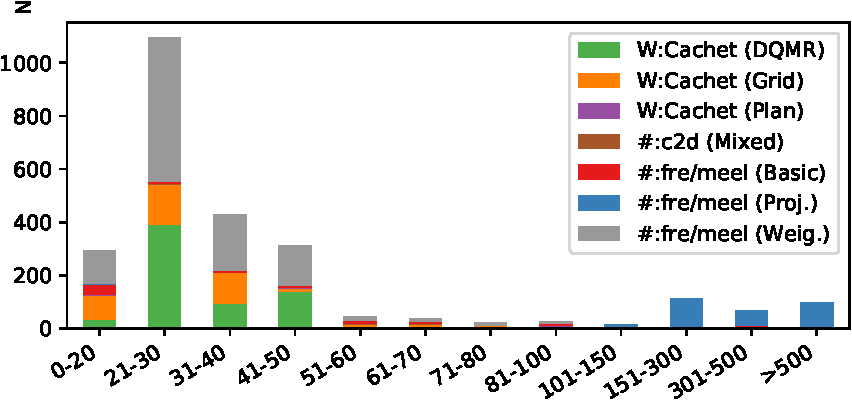
\includegraphics{0-figs/width}
%     %
%   }%
%   \\
%   Decomposition Heuristic:
%   \begin{itemize}
%   \item  Runtime well below a second (max. 2.5) 0--40
%   \item Timeout (900s) on 41 instances
%   \item[\Ra] 54\% primal treewidth below 30; 70\% below 40
%   \end{itemize}
% \end{frame}

\begin{frame}{\#SAT: Width Comparison (Preprocessing comp.)}
  \bigskip\bigskip%
  {\centering
    \includegraphics[width=.90\columnwidth]{1-plots/plots_Width/plot_Width.pdf}}\\
  \centering
  \begin{itemize}
  \item  Runtime well below a second (max. 2.5s) 0-40; timeout (1800s)
  %\item Timeout (900s) on 41 instances
  \item[\Ra] 54\% primal treewidth below 30; 70\% below 40
  \item[$\Rightarrow$] Preprocessing produces TDs of significantly smaller
    width
  \end{itemize}
  %\alert{$\Rightarrow$ Produce decompositions of significantly smaller width}
\end{frame}


\begin{frame}{WMC: Width Comparison}% (w/o Preprocessing)}
  \bigskip\bigskip%
  {\centering
    \includegraphics[width=.90\columnwidth]{1-plots/plots_Width_w/plot_Width.pdf}}\\
  \centering
  \alert{$\Rightarrow$ Produce decompositions of significantly smaller width}
\end{frame}


\begin{frame}{Experimental Work (Runtime)}
  \begin{block}{Setting (Runtime Comparison)}
    Take \gpusatone, \gpusatnu, and versions as well as sequential and
    parallel solvers.\\
    Consider Wallclock
  \end{block}

    \begin{block}{Hardware}
    \begin{itemize}
    \item non-GPU solving: cluster of 9 nodes; each two E5-2650
      CPUs (12cores) 2.2 GHz, 256 GB RAM; disabled HT, kernel~4.4
    \item GPU-solving: i3-3245 3.4 GHz; 16 GB RAM; GPU: Sapphire Pulse
      ITX Radeon RX 570 GPU; 1.24 GHz with 32 compute units, 2048
      shader units, 4GB VRAM
    \end{itemize}
  \end{block}
\end{frame}

% \begin{frame}{Experimental Work (Runtime Disclaimer)}
%   \vspace{3em}
%   \begin{itemize}
%   \item Parallization not obvious
%   \item Application is important
%   \item GPU a good hardware accellerator for parallelization
%   \item BUT does not fit into the standard SAT solver box 
%   \end{itemize}
% \end{frame}

\begin{frame}{Experimental Work (Runtime Disclaimer)}
  \begin{block}{Questionable Setting?}
    Aren't you comparing apples and oranges? YES.
  \end{block}
  \begin{block}{Problems of the Setting}
    \begin{itemize}
    \item We compare on different hardware
    \item[$\Ra$] Soon, new cluster node with the same specs and two
      GPUs
    \item Wallclock is unfair
    \item[] Usually user is interested in getting things done
      quickly (+ fairly cheap)
    \item[$\Ra$] Power consumption (Joule) and price of investment
      better measure\\ (BUT not accessible with the current framework)
    \item[$\Ra$] We use cheap consumer hardware (200\$) for the GPU\\
      not a Tesla K80 (8k\$) or DGX2 (400k\$)
    \item Parallel vs. sequential: No excuse, sorry
    \end{itemize}
  \end{block}
\end{frame}


\begin{frame}[shrink=1]{\#SAT}
\centering

\begin{table}[t]
  \centering
  \resizebox{.8\columnwidth}{!}{%
    \begin{tabular}{{l|lH||rrrrrrrr||r||rHr}}
      \toprule
      & solver & racc & 0-20 & 21-30 & 31-40 & 41-50 & 51-60 & $>$60 & best & unique & $\sum$ & time[h] & rank \\
      \midrule
      \parbox[t]{1em}{\multirow{9}{*}{\rotatebox[origin=c]{90}{pmc preprocessing}}}&miniC2D & \textbf{0} & 1193 & 29 & \textbf{10} & 2 & 1 & 7 & 13 & 0 & \textbf{1242} & \textbf{68.77} & 1 \\
      &\gpusatnu & 4.7E-15 & \textbf{1196} & \textbf{32} & 1 & 0 & 0 & 0 & 250 & %1/
                                                                                     \textbf{8} & 1229 & 71.27 & 2 \\
      &d4 & \textbf{0} & 1163 & 20 & \textbf{10} & 2 & \textbf{4} & 28 & 52 & 1 & 1227 & 76.86 & 3 \\
      & \gpusatnuv{A+B} & {4.6E-15} & {1187} & 18 & 1 & 0 & 0 & 0 & 120 & 7 & 1206 & 74.56 & 4 \\
      &countAntom 12 & \textbf{0} & 1141 & 18 & \textbf{10} & \textbf{5} & \textbf{4} & 13 & 101 & 0 & 1191 & 84.39 & 5 \\
      &c2d & \textbf{0} & 1124 & 31 & \textbf{10} & 3 & 3 & 10 & 20 & 0 & 1181 & 84.41 & 6 \\
      &sharpSAT & \textbf{0} & 1029 & 16 & \textbf{10} & 2 & \textbf{4} & \textbf{30} & \textbf{253} & 1 & 1091 & 106.88 & 7 \\
      &\gpusatone & 1.7E-13 & 1020 & 16 & 0 & 0 & 0 & 0 & 106 & 7 & 1036 & 114.86 & 8 \\
      & sdd & \textbf{0} & 1014 & 4 & 7 & 1 & 0 & 2 & 0 & 0 & 1028 & 124.23 & 9 \\
      % \textit{sts} & \inacc{2.7} & \inacc{927} & \inacc{4} & \inacc{8} & \inacc{\textbf{7}} & \inacc{\textbf{5}} & \inacc{\textbf{52}} & \inacc{73} & \inacc{\textbf{21}} & \inacc{1003} & \inacc{128.43} & 9 \\
      % & dsharp & 4.4E-6 & 853 & 3 & 7 & 2 & 0 & 0 & 84 & 0 & 865 & 157.87 & 10 \\
      \midrule
      & solver & racc & 0-20 & 21-30 & 31-40 & 41-50 & 51-60 & $>$60 & best & unique & $\sum$ & time[h] & rank \\
      % \midrule
      % \parbox[t]{1em}{\multirow{8}{*}{\rotatebox[origin=c]{90}{B+E preprocessing}}}&c2d & \textbf{0} & 1199 & 24 & \textbf{9} & 0 & 2 & 23 & 14 & 0 & \textbf{1257} & \textbf{63.46} & 1 \\
      % &miniC2D & \textbf{0} & 1203 & \textbf{27} & 8 & 0 & 2 & 12 & 8 & 0 & 1252 & 64.92 & 2 \\
      % &d4 & \textbf{0} & 1182 & 15 & \textbf{9} & \textbf{1} & \textbf{3} & 31 & 79 & 1 & 1241 & 69.32 & 3 \\
      % &countAntom 12 & \textbf{0} & 1177 & 14 & 8 & 0 & 2 & \textbf{34} & 100 & 0 & 1235 & 69.79 & 4 \\
      % &\gpusatnu & 6.4E-16 & \textbf{1204} & 26 & 1 & 0 & 0 & 0 & \textbf{150} & \textbf{3} & 1231 & 68.15 & 5 \\
      % &\gpusatnuv{A+B} & {6.4E-16} & 1201 & 21 & 1 & 0 & 0 & 0 & 67 & \textbf{3} & 1223 & 70.39 & 6 \\
      % &sdd & \textbf{0} & 1106 & 11 & 4 & \textbf{1} & 1 & 4 & 0 & 0 & 1127 & 100.48 & 7 \\
      % &\gpusatone & 9.9E-12 & 1037 & 16 & 0 & 0 & 0 & 0 & 87 & %0/
      %                                                          \textbf{3} & 1053 & 110.87 & 8 \\
      %                                                          % \textit{sts} & \inacc{1.3} & \inacc{943} & \inacc{10} & \inacc{5} & \inacc{\textbf{1}} & \inacc{\textbf{3}} & \inacc{\textbf{49}} & \inacc{21} & \inacc{\textbf{15}} & \inacc{1011} & \inacc{125.58} & \inacc{8} \\
      % &bdd\_minisat\_all & \textbf{0} & 926 & 6 & 3 & \textbf{1} & 1 & 0 & 101 & 0 & 937 & 140.59 & 9 \\
      % % &sharpSAT & \textbf{0} & 842 & 14 & 8 & 0 & 2 & \textbf{35} & \textbf{197} & 1 & 901 & 153.65 & 10 \\
      % \midrule
      % &solver & racc & 0-20 & 21-30 & 31-40 & 41-50 & 51-60 & $>$60 & best & unique & $\sum$ & time[h] & rank \\
      % \bottomrule
      \midrule
      \parbox[t]{1em}{\multirow{9}{*}{\rotatebox[origin=c]{90}{without preprocessing}}}& countAntom 12 & \textbf{0} & 118 & 511 & 139 & \textbf{175} & \textbf{21} & \textbf{181} & 318 & 15 & \textbf{1145} & \textbf{96.64} & 1 \\
      & d4 & \textbf{0} & 124 & 514 & 148 & 162 & \textbf{21} & 168 & 69 & 15 & 1137 & 104.94 & 2 \\
      & c2d & \textbf{0} & 119 & 525 & \textbf{165} & 161 & 18 & 120 & 48 & 15 & 1108 & 110.53 & 3 \\
      & miniC2D & \textbf{0} & 122 & 514 & 128 & 149 & 9 & 62 & 0 & 0 & 984 & 141.22 & 4 \\
      & sharpSAT & \textbf{0} & 100 & 467 & 124 & 156 & 12 & 123 & \textbf{390} & 4 & 982 & 135.41 & 5 \\
      % &\textit{sts} & \inacc{1.02} & \inacc{118} & \inacc{466} & \inacc{75} & \inacc{\textbf{196}} & \inacc{11} & \inacc{44} & \inacc{217} & \inacc{\textbf{58}} & \inacc{910} & \inacc{150.79} & \inacc{6} \\
      % &gpusat2(vbest) & {9.8E-18} & \textbf{125} & \textbf{539} & 98 & 141 & 0 & 0 & 97 & %0/
      % \textbf{21} & 903 & 149.75 & 7 \\
      & \gpusatnuv{A+B} & {9.8E-18} & \textbf{125} & \textbf{539} & 96 & 138 & 0 & 0 & 94 
                                                                            & \textbf{19} & 898 & 151.16 & 8 \\
                                                                            % &\gpusatnuv{A} & {9.8E-18} & \textbf{125} & \textbf{539} & 83 & 139 & 0 & 0 & 96 & 
                                                                            % 0/
                                                                            % 19 & 886 & 153.28 & 9 \\
                                                                            % &\gpusatnuv{B} & {9.8E-18} & \textbf{125} & 523 & 96 & 138 & 0 & 0 & 78 & %0/
                                                                            % 17 & 882 & 155.43 & 10 \\
      &\gpusatnu & 9.7E-18 & \textbf{125} & 523 & 96 & 138 & 0 & 0 & 78 & 17 & 882 & 155.43 & 8 \\
      &\gpusatone & 1.4E-10 & \textbf{125} & 524 & 67 & 140 & 0 & 0 & 82 & %1/
                                                                           9 & 856 & 162.03 & 11 \\
      &cachet & \textbf{0} & 99 & 430 & 71 & 152 & 8 & 57 & 3 & 0 & 817 & 176.26 & 12 \\
      %&dsharp & 4.4E-6 & 100 & 382 & 57 & 135 & 7 & 5 & 73 & 0 & 686 & 205.31 & 13 \\
      \midrule
      &solver & racc & 0-20 & 21-30 & 31-40 & 41-50 & 51-60 & $>$60 & best & unique & $\sum$ & time[h] & rank \\
      \bottomrule
    \end{tabular}
  }
%   \caption{%
%     Number of~\cSAT instances (grouped by treewidth upper bound intervals)
%     solved by sum of the top five sequential and all parallel counting solvers 
%     with preprocessor pmc (top), B+E (mid), and without preprocessing (bottom).
%     time[h] is the cumulated  wall clock time in hours, where unsolved instances 
%     are included with 900 seconds.
% %
%   }%
%   \label{tab:sat:merged}
%
\end{table}%
\end{frame}



\begin{frame}{\#SAT: Runtime Results (w. Preprocessing)}
  \centering
  \resizebox{.8\columnwidth}{!}{%
    \includegraphics{1-plots/plot_pmc_enlarged}
    %
  }%
  \\
%  \includegraphics[width=.8\columnwidth]{1-plots/1-plots_width_legend/plots_pmc/plot_pmc_enlarged.pdf}\\
\centering
$\Rightarrow$ Techniques pay off after preprocessing
\end{frame}


\begin{frame}[shrink=1]{WMC}
\begin{table}[t]
  \centering
  \resizebox{.8\columnwidth}{!}{%
    \begin{tabular}{{l|lH||rrrrrrrr||r||rHr}}
      \toprule
& solver & racc & 0-20 & 21-30 & 31-40 & 41-50 & 51-60 & $>$60 & best & unique & $\sum$ & time[h] & rank \\
      \midrule\midrule
      %\textit{sts} & \inacc{2.9E+5} & \inacc{820} & \inacc{170} & \inacc{\textbf{24}} & \inacc{\textbf{27}} & \inacc{\textbf{0}} & \inacc{\textbf{4}} & \inacc{174} & \inacc{\textbf{47}} & \inacc{\textbf{1045}} & \inacc{23.57} & 1 \\
      \parbox[t]{1em}{\multirow{5}{*}{\rotatebox[origin=c]{90}{with pmc*}}} & miniC2D & 1 & 858 & \textbf{164} & \textbf{6} & \textbf{0} & \textbf{0} & 3 & 13 & \textbf{8} & \textbf{1031} & 21.29 & 2 \\
      & \gpusatone & 4.4E-6 & \textbf{866} & 158 & 0 & \textbf{0} & \textbf{0} & 0 & \textbf{348} & 4 & 1024 & 18.03 & 3 \\
      %gpusat2 vbest & 4.4E-6 & 866 & 156 & 0 & 0 & 0 & 0 & 48 & 0/4 & 1022 & 17.86 & 5 \\
      & \gpusatnuv{A+B} & 4.4E-6 & \textbf{866} & 156 & 0 & \textbf{0} & \textbf{0} & 0 & 343 & {4} & 1022 & \textbf{17.86} & 4 \\
      & \gpusatnu & 4.4E-6 & \textbf{866} & 138 & 0 & \textbf{0} & \textbf{0} & 0 & 299 & 4 & 1004 & 22.43 & 4 \\
      %gpusat2 array & 4.4E-6 & 866 & 156 & 0 & 0 & 0 & 0 & 25 & 0/4 & 1022 & 17.86 & 4 \\
      %gpusat2 tree & 4.4E-6 & 866 & 138 & 0 & 0 & 0 & 0 & 23 & 0/4 & 1004 & 22.43 & 7 \\
      & d4 & \textbf{0} & 810 & 106 & 0 & \textbf{0} & \textbf{0} & 0 & 46 & 0 & 916 & 55.36 & 5 \\
      %d4+d-DNNF  & 1.6E-4 & 760 & 53 & 0 & 0 & 0 & 1 & 371 & 0 & 814 & 69.83 & 9 \\
      & cachet & \textbf{0} & 617 & 128 & 1 & \textbf{0} & \textbf{0} & 3 & 106 & 1 & 749 & 93.65 & 6 \\
      \midrule
      \midrule
      %\textit{sts} & \inacc{6.0E+5} & \inacc{80} & \inacc{\textbf{529}} & \inacc{\textbf{190}} & \inacc{\textbf{208}} & \inacc{1} & \inacc{6} & \inacc{\textbf{260}} & \inacc{\textbf{90}} & \inacc{\textbf{1014}} & \inacc{\textbf{34.53}} & 1 \\
      \parbox[t]{1em}{\multirow{5}{*}{\rotatebox[origin=c]{90}{without pre}}}& d4 & 5.8E-5 & 82 & 501 & \textbf{142} & \textbf{156} & \textbf{10} & \textbf{19} & 111 & \textbf{24} & \textbf{910} & \textbf{53.97} & 2 \\
& miniC2D & 1 & 84 & 517 & 134 & 152 & 3 & 4 & 19 & 7 & 894 & 59.69 & 3 \\
      %gpusat2 vbest & 4.4E-6 & 86 & 527 & 100 & 141 & 0 & 0 & 81 & 0/22 & 854 & 63.03 & 4 \\
      & \gpusatnuv{A+B} & 4.4E-6 & \textbf{86} & \textbf{527} & 98 & 138 & 0 & 0 & 167 & {19} & 849 & 64.40 & 4 \\	
      & \gpusatnu & 4.4E-6 & \textbf{86} & 511 & 98 & 138 & 0 & 0 & 131 & 7 & 833 & 68.61 & 4 \\
      %gpusat2 tree & 4.4E-6 & 86 & 511 & 98 & 138 & 0 & 0 & 0 & 0/17 & 833 & 68.61 & 6 \\
      %gpusat2 array & 4.4E-6 & 86 & 527 & 81 & 139 & 0 & 0 & 81 & 0/19 & 833 & 66.01 & 7 \\
      & \gpusatone & 4.4E-6 & \textbf{86} & 513 & 68 & 140 & 0 & 0 & \textbf{182} & 10 & 807 & 73.78 & 5 \\
      %d-DNNF-r.  & 1.6E-3 & 77 & 447 & 116 & 141 & 9 & 5 & 363 & 0 & 795 & 78.49 & 9 \\
      & cachet & \textbf{0} & 60 & 447 & 100 & 145 & 2 & 9 & 118 & 1 & 763 & 89.80 & 6 \\
      \bottomrule
    \end{tabular}
  }
\end{table}
\end{frame}

% \begin{frame}{\#SAT: Runtime Results (wo. Preprocessing)}
%  \centering \includegraphics[width=.8\columnwidth]{1-plots/1-plots_width_legend/plots_wo-pre/plot_wo-pre_enlarged.pdf}
% \end{frame}


% \begin{frame}{\#WMC: Runtime Results (w. Preprocessing)}
%   \centering
%   \includegraphics[width=.8\columnwidth]{1-plots/1-plots_width_legend/plots_w_pmc/plot_w_pmc_enlarged.pdf}\\
%   \centering
%   $\Rightarrow$: After preprocessing \#SAT no3, WMC no2
% \end{frame}


\begin{frame}{Summary}
  \begin{block}{Contributions}
    \begin{itemize}
    \item Established Architecture for DP on the GPU
    \item Competitive Implementation for \#SAT/WMC solving
    \end{itemize}
  \end{block}
  \begin{block}{Benchmark: Comparing apples and oranges}
    BUT: you compare parallel and sequential solvers.
    \begin{enumerate}
    \item We run on cheap consumer hardware (200\$)
    \item Cannot measure speedup due to OpenCL/display driver limitations\\
      $\Rightarrow$ migrate to cuda
    \end{enumerate}
  \end{block}
\end{frame}

\begin{frame}{Summary cont.}
  \begin{block}{Take Home Messages}
    \begin{enumerate}
    \item Parameterized Algorithms can actually work\\
      (Preprocessing is key; some techniques pay only off with right
      preprocessing)
      \item Does it ``work'' for SAT? $\Rightarrow$ we don't expect so.
    \end{enumerate}
  \end{block}
  
  \begin{block}{Future Work}
    \begin{itemize}
    \item Improve current setup by: \\
      Portfolio solving; Parallel Usage of GPUs; Alternative
      Frameworks
    \item Consider whether stable among different GPU hardware
    \item Parameters (pswidth)
    \end{itemize}
  \end{block}
  \vspace{-0.5em}
  \only<2>{
    \centering
    \alert{%
    Thanks for listening!
    %
    }\medskip\\
    
    % {\color{red}
    %   Advertisement:\\
    %   PACE-2019 (vertex cover and hypertree decompositions)\\
    % {\footnotesize{}GitHub:daajoe/\{benchmark-tool,fhtd,trellis\}}}
    
    %
    \bigskip
    %
  }
  %\alert{Who is interested in collaborating?}
  
  Sponsors: FWF Y698 \& P26696; DFG HO 1294/11-1
\end{frame}


\begin{frame}{References}
  \hangpara{5em}{1}[AMW'17]: Abseher, Musliu, Woltran. htd -- A Free,
  Open-Source Framework for (Customized) Tree Decompositions and
  Beyond. CPAIOR'17. 2017. doi: 10.1007/978-3-319-59776-8\_30

  \hangpara{5em}{1}[FHWZ'18]: Fichte, Hecher, Woltran, Zisser. Weighted
  Model Counting on the {GPU} by Exploiting Small
  Treewidth. ESA'18. 2018. doi: 10.4230/LIPIcs.ESA.2018.28

  \hangpara{4.5em}{1}[FHZ'19]: Fichte, Hecher, Zisser. gpusat2 -- An
  Improved GPU Model Counter. CP 2019.

  \hangpara{8.5em}{1}[SamerSzeider'10]: Samer, Szeider. Algorithms for
  propositional model counting. JDA. 2010. doi:
  10.1016/j.jda.2009.06.002
  \bigskip\bigskip

  gpusat is available at: \url{https://github.com/daajoe/gpusat}
\end{frame}


% \begin{frame}[label=questions,noframenumbering]{}
%   \bigskip
%   \bigskip
%   \bigskip
%   \bigskip
%   \bigskip
%   \bigskip
%   \bigskip
%   \begin{center}
%     \alert{\Huge Questions?}
%   \end{center}
%   \bigskip
%   \bigskip
%   \bigskip
%   \bigskip
%   \bigskip
%   \bigskip  
%   \bigskip  
%   \bigskip  
%  \hfill\hyperlink{backup_slides<1>}{\beamergotobutton{Backup Slides}}
% \end{frame}


\beginbackup
\subsection{Backup}

\begin{frame}[label=questions,noframenumbering]{}
  \bigskip
  \bigskip
  \bigskip
  \bigskip
  \bigskip
  \bigskip
  \bigskip
  \begin{center}
    \alert{\Huge Backup Slides}
  \end{center}
  \bigskip
  \bigskip
  \bigskip
  \bigskip
  \bigskip
  \bigskip  
  \bigskip  
  \bigskip  
\end{frame}



\begin{frame}{Solving (Width: 0--30): \#SAT}
  \begin{columns}[T]
    \begin{column}{0.8\textwidth}
      \resizebox{1\columnwidth}{!}{%
        \includegraphics{0-figs/Plot_CSAT_0-30}
        % 
      }
    \end{column}
    \begin{column}{0.2\textwidth}
      \alert{kc/cdcl}: c2d, d4, dsharp\\
      \alert{dp}: gpusat, dynQBF, dynasp\\
      \alert{parallel}: countAntom, gpusat\\
      \alert{cdcl}: Cachet, sharpSAT, clasp\\
      \alert{bdd}: sdd\\
      \alert{approx}: approxmc, sts
    \end{column}
  \end{columns}
\end{frame}


\begin{frame}{Solving: \#SAT}
%\vspace{-2em}
\begin{table}%[h]
\resizebox{\columnwidth}{!}{%
\begin{tabular}{{l@{~}||H@{~}H@{~}r@{~~}r@{~~}r@{~~}r@{~~}r@{~~}r||r@{~~}|rr}}
\toprule
            solver &           avg &   acc &      0-20 &     21-30 &     31-40 &     41-50 &    51-60 &     $>$60 &      best &     $\sum$ &  rank \\
\midrule
%          approxmc &            na &    na &        13 &        10 &        10 &         1 &        1 &        44 &        11 &    $^*$103 &    20 \\
% bdd\_minisat\_all &            na &    na &        39 &        95 &        26 &        28 &        1 &        15 &         6 &    $^*$243 &    18 \\
               c2d &  1.850000e-10 &  0.0 &       164 &  \ts{519} &  \tm{175} &       116 &  \ts{20} &       118 &       120 &  \ts{1112} &     2 \\
            Cachet & -2.463054e-03 & -0.0 &       133 &       421 &        91 &       109 &        8 &        58 &        13 &        820 &     7 \\
%          cnf2eadt &            na &    na &        78 &       193 &        50 &        57 &        8 &        54 &        45 &    $^*$528 &    17 \\
                d4 &  1.850000e-10 &  0.0 &  \tm{169} &       510 &  \ts{156} &  \ts{119} &  \tm{23} &  \tm{162} &       191 &  \tm{1139} &     1 \\
%            dsharp &            na &    na &       134 &       356 &        71 &        97 &        7 &         6 &        69 &    $^*$806 &    11 \\
%         dynasp(i) &            na &    na &       166 &       258 &         0 &         0 &        0 &         1 &         3 &    $^*$592 &    15 \\
%         dynasp(p) &            na &    na &  \ts{167} &       252 &         0 &         0 &        0 &         1 &        13 &    $^*$588 &    16 \\
%           dynqbfa &            na &    na &       135 &       331 &        80 &        68 &        0 &         6 &         0 &    $^*$756 &    12 \\
%           dynqbfe &            na &    na &       134 &       333 &        81 &        67 &        0 &         6 &         0 &    $^*$756 &    12 \\
%         gpusat(i) &  3.220000e-10 &  0.0 &  \tm{169} &       490 &        79 &        97 &        0 &         0 &         1 &        835 &     8 \\
%        gpusat(i4) &  5.090000e-10 &  0.0 &       168 &       427 &        70 &        89 &        0 &         0 &         1 &    $^*$761 &    14 \\
         gpusat(p) &  3.640000e-10 &  0.0 &  \tm{169} &  \tm{523} &        79 &       104 &        0 &         0 &        88 &        875 &     6 \\
%        gpusat(p4) &  3.030000e-10 &  0.0 &  \tm{169} &       478 &        79 &        97 &        0 &         0 &         0 &        823 &     7 \\
           miniC2D &  2.560000e-10 &  0.0 &  \ts{167} &       491 &       137 &       103 &        8 &        67 &         2 &        973 &     4 \\
%               sdd &            na &    na &       142 &       339 &       113 &        75 &        5 &         5 &         0 &        822 &    10 \\
%         sharpCDCL &            na &    na &        21 &        83 &        20 &        24 &        1 &        44 &         9 &    $^*$225 &    19 \\
          sharpSAT &            na &    na &       136 &       465 &       136 &       112 &       11 &  \ts{124} &  \tm{483} &       984 &     3 \\
               sts & -1.116004e-01 & -0.1 &       162 &       448 &       101 &  \tm{146} &       10 &        45 &  \ts{252} &        912 &     5 \\
\bottomrule
\end{tabular}
}
\caption{Number of counting instances solved by solver and interval.%by sum of the top ten counting solvers %and 
%  gpusat. 
%The symbol~$^*$ indicates that this gpusat configuration was not among the top ten.
%
}%
\label{fig:solved-count}
\end{table}
\end{frame}


% \begin{frame}{Solving (Width: 0--30): WMC}
%   \resizebox{1.04\columnwidth}{!}{%
%     % \resizebox{0.5\columnwidth}{!}{%
%     \includegraphics{0-figs/Plot_WMC_0-30}
%     % 
%   }
% \end{frame}


\begin{frame}{Empirical Work (first approach)}%{Summary (Empirical Work)}
  \bigskip
  \bigskip
  \begin{block}{Observations}
    \begin{itemize}
    \item Implementation is fairly naive
    \item Still: competitive up to width 30
    \item Requirement: obtain decompositions fast
    \item Width was surprisingly small (different for SAT)
    \end{itemize}
  \end{block}
  % \medskip
  % \begin{block}{Future Work}
  %   \begin{itemize}
  %   \item Evaluation of other PACE solvers
  %   \item Effect of Preprocessing
  %   \item ...
  %   \end{itemize}
  %   \end{block}
\end{frame}

\section{Bibliography}


% \begin{frame}[fragile,allowdisplaybreaks,allowframebreaks,label=bib]{References}
%   \bibliography{/Users/fichte/Literature/johannes}
% \end{frame}

%\makereferences{../literature}


% \begin{frame}[noframenumbering,label=backup_slides]{Backup Slides}
% \end{frame}
\section{Backup Slides}


\begin{frame}{Implementation Ideas (cont.)}
  \begin{block}{(1) Data Structures}
    \begin{enumerate}
    \item[b.] BST (details):
      \begin{itemize}
      \item Continuous sequence 64-bit unsigned integers (cells)
      \item Cell: empty, index, and value (counter)
      \item index cells: lower 32 bits index to the next cell\\
        (lower bits assingment 0, upper 1)
      \item Handle Sync (between parallel threads) by keeping track of
        the current size (number of allocated cells; prevent to
        allocate cell again)
      \end{itemize}
    \end{enumerate}
  \end{block}
\end{frame}



\begin{frame}[label=algorithm]{Algorithm for Primal Graph}
  \resizebox{0.8\textwidth}{!}{%
    \centering
     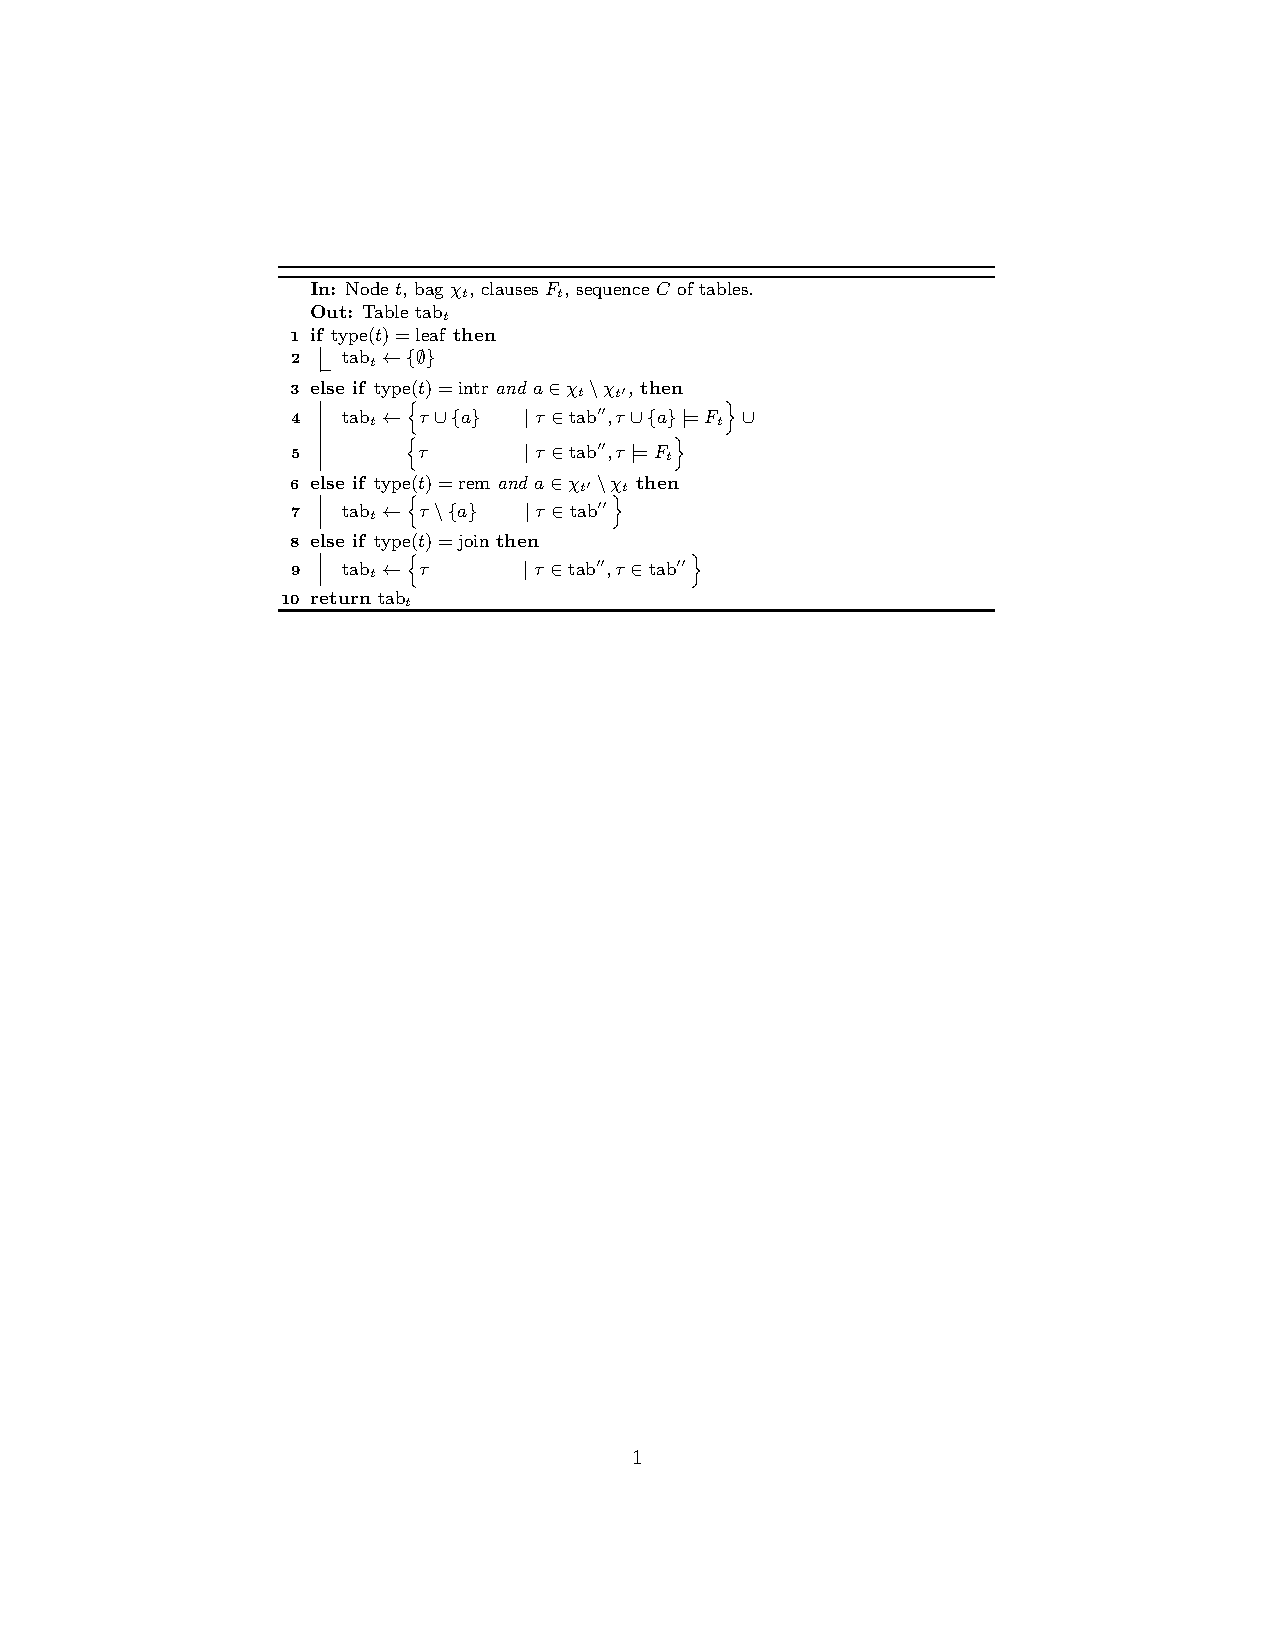
\includegraphics[trim={3.5cm 15cm 8cm 4cm},clip]{2-includes/sat_algo.pdf}
   }
\end{frame}



\backupend

\end{document}

%%% Local Variables:
%%% mode: latex
%%% TeX-engine: xetex
%%% TeX-master: t
%%% End: